\documentclass{report}
\usepackage{graphicx}
\usepackage[a4paper, total={6in, 8in}]{geometry}
\usepackage{amsmath}
\usepackage[hidelinks]{hyperref}
\usepackage{tabu}
\usepackage{float}
\usepackage{listings}
\usepackage{color}
%\usepackage[toc,page]{appendix}
\usepackage[title]{appendix}
\usepackage{enumitem}
%\usepackage{fancyhdr}

\graphicspath{{figures/}}

\newlist{abbrv}{itemize}{20}
\setlist[abbrv,1]{label=,labelwidth=1in,align=parleft,itemsep=0.1\baselineskip,leftmargin=!}

%\pagestyle{fancy}
%\lhead{This is my name}
%\rhead{LOCATION BASED\\ AUTHENTICATION USING \\WI-FI SIGNAL STRENGTH}
%\cfoot{right of the footer!}
%\renewcommand{\headrulewidth}{0.1pt}
%\renewcommand{\footrulewidth}{0.4pt}


\setcounter{secnumdepth}{3}
\begin{document}

	\pagenumbering{gobble}
		
	\begin{titlepage}
    \begin{center}
        \vspace*{0.1cm}
        
        \begin{figure}[h]
        	\centering
        	
\includegraphics[width=0.2\textwidth]{uoc_logo.png}
        \end{figure}
        
        %\newline
        \Huge
        \textbf{VISUAL LIGHT COMMUNICATION FOR LOCATION BASED Wi-Fi CONNECTIVITY}
        

        
        \vspace{1.5cm}
        
        \large
        \textbf{J.A.R.N. CHANDRATHILAKA}
        
        \vfill
        
        A thesis presented for the degree of\\
        Master of Computer Science
        
        \vspace{0.8cm}
        
        %\includegraphics[width=0.4\textwidth]{university}
        
        University of Colombo School of Computing\\
        Sri Lanka\\
        2018
        \begin{figure}[h]
        	\centering
        	
\includegraphics[width=0.2\textwidth]{ucsc.jpg}
        \end{figure}
        
    \end{center}
\end{titlepage}
	
	\newpage
	\pagenumbering{roman}
		
	\chapter*{DECLARATION}
	\addcontentsline{toc}{chapter}{DECLARATION}
I hereby declare that I have carried out this LOCATION BASED AUTHENTICATION USING WI-FI SIGNAL STRENGTH research project by myself for the MIS3104 – Individual Project for Master of Science in Information Security course.\\
\newline
\newline
Student's Name : Jayaweera Arachchige Randeepa Nisal Chandrathilaka\\
\newline
Student's Signature :..............................\\
\newline                   
Date :...........................\\
\newline
\newline
Supervisor's Name : Dr. Kasun De Zoysa\\
\newline
Supervisor's Signature :...........................\\
\newline
Date :............................
	
	\chapter*{ACKNOWLEDGMENT}
	\addcontentsline{toc}{chapter}{ACKNOWLEDGMENT}
As a final year student of the Master of Science in Information Security,University of Colombo School of Computing, Sri Lanka, I am taking this occasion to express my gratitude to the University of Colombo School of Computing and also the people who helped me to be success with this project.
\paragraph{}
I would like to express my gratitude to my project supervisor, Dr.Kasun De Zoysa, Senior lecturer in the University of Colombo School of Computing, who helped me and guided me with valuable suggestions throughout the entire project.
And also I would like to express my gratitude to my dear parents and my dear brothers who helped me to complete this project and Master of Sciences in Information Security degree program in various ways and the encouragement which was given to me.
Finally I would like to express my gratitude to all the people who helped me throughout this project and gave support to me by various ways. 	
	
	\chapter*{ABSTRACT}
	%\begin{abstract}
\addcontentsline{toc}{chapter}{ABSTRACT}
Authentication is the process of identifying the user as genuine for the system
which is a key functionality, when considering the security of all systems. The
most conventional way of authentication depends on the user name and
password. Even though the three(03)acceptable concepts which are used to
authenticate users: something user knows(password), something user has (tokens, cards)
and something user is (bio-metrics) or the combination of them are used, the systems are
still vulnerable of being attacked by the hackers which results huge impact on
cost, reputation of the organization and privacy of the users/ customers.
Even though, additional security layers together with traditional authentication
methods have already been introduced, still there is a need of a solution which
is capable of providing secure authentication mechanism which is compatible
with existing infrastructure without requesting special equipments.
Wi-Fi access points are available in most of the places which provide connectivity
to the systems in a particular area and most of the authorized professionals who
are responsible for most critical functionalities of the systems widely use Wi-Fi access point to
gain access to the servers, so as the hackers by spoofing their actual identity by
pretending as a genuine user to misuse data.
To address this problem, the research project LOCATION BASED AUTHENTICATION USING WI-FI
SIGNAL STRENGTH tries to introduce an additional security layer to the Wi-Fi access point without
requesting special equipments and it additionally checks the location where user tries to access the system with respect to Wi-Fi signal strength together with the combination of user name and password to enforce the security policy.

%\end{abstract}
	
	
	\tableofcontents
	\addcontentsline{toc}{chapter}{TABLE OF CONTENTS}
	
	
	\listoffigures
	\addcontentsline{toc}{chapter}{LIST OF FIGURES}
	
	
	\listoftables
	\addcontentsline{toc}{chapter}{LIST OF TABLES}
	
	\chapter*{LIST OF ABBREVIATIONS}
	\chaptermark{LIST OF ABBREVIATIONS}
	
	\begin{abbrv}
		
		\item[IEEE]				The Institute of Electrical and Electronic Engineers
		\item[Wi-Fi]			IEEE 802.11 standards (Wi-Fi Technology)
		\item[AP]				Access Point
		\item[RC4]				Rivest Cipher 4
		\item[CPU]				Central Processing Unit
		\item[e-Commerce]		Electronic Commerce
		\item[e-Tailling]		Electronic Retailing
		\item[RADIUS]			Remote Authentication Dial-In User Service
		\item[PII]				Personally Identifiable Information
		\item[IV]				Initialization Vector
		\item[NFC]				Near Field Communication	
		\item[API]				Application Programming Interface
		\item[IoT]				Internet of Things
		\item[BYOD]				Bring Your Own Device
		\item[PAP]				Password Authentication Protocol
		\item[CHAP]				Challenge Handshake Protocol
		\item[WEP]				Wired Equivalent Privacy
		\item[WPA]				Wi-Fi Protected Access
		\item[WPA2]				Wi-Fi Protected Access Version2	
		\item[WPA3]				Wi-Fi Protected Access Version3
		\item[EAP]				Extensible Authentication Protocol
		\item[TKIP]				Temporal Key Integrity Protocol
		\item[MIC]				Message Integrity Check
		\item[CRC]				Cyclic Redundancy Check
		\item[GPS]				Global Position System
		\item[LED]				Light Emitted Diode
		\item[VLC]				Visible Light Communication
		\item[RSSI]				Received Signal Strength Indicator
		\item[2D]				2 - Dimensions
		\item[3D]				3 - Dimensions
		\item[IPV4]				Internet Protocol Version 4
		\item[IPV6]				Internet Protocol Version 6
		\item[JSON]				Java Script Object Notation
		\item[AES]				Advanced Encryption Standard
	\end{abbrv}
	\addcontentsline{toc}{chapter}{LIST OF ABBREVIATIONS}
	
	\newpage
	\pagenumbering{arabic}

	\chapter{INTRODUCTION}
	\section{INTRODUCTION}
Technology, in nowadays plays a major role in each corner of the world and expects the continuous growth. Any person, any business, any service is now interacted with technology, somehow, either fully or up to some extent. The beauty of the technology is that it always changes with new researches and  findings all around the world. People do their researches to test new concepts and introduce new findings to the world to make life easier. With the  introduction of new technologies, market has become really competitive and opens the door to the entire world. People have realized that it is not easy to survive their businesses without having technology. Not only the business world, human life style has also become really closed with the technology and some life styles have been entirely changed due to new technologies. With the broad development of technology, organizations tend to acquire new technologies to the business process, which becomes a new business itself. Even most critical businesses such as financial, industrial also acquire new technologies because of the business competition and for their effectiveness. In order to keep customers, business has to provide the best competitive service to the customer which becomes really pain without new technologies. No matter what kind of business it is, technology is everywhere. 

\paragraph{}
Technology runs our lives these days. Smart phones, tablets and computers \verb|-| we really can't seem to function without them. In a very short amount of time, technology has exploded in the market and now, many people cannot imagine a life without it.  All technologies are born out of purpose. For example, search engines were created to sort through the massive amounts of data online. With the introduction of each new technology, the existing technologies were replaced and the new technologies were able to create something better than what was previously used. And on and on it goes. It has become an integral part of our daily life. We are almost surrounded by technology and we always use technology everywhere and all the time. Computer and internet technologies have changed sectors like medicine, tourism, education, entertainment etc... Technology has touched every aspect of life, making it easier, better and different. It has affected the human life and has changed our living.\cite{technology}

\paragraph{}
Most of the businesses depend on the computer technology as it gives a helping hand to develop and maintain the business. Technology has important effects on business operations. No matter the size of the enterprise, technology has both tangible and intangible benefits that will help to make money and customers. Technological infrastructure affects the culture efficiency and relationships of a business.

\paragraph{Why is technology important in businesses?}
\begin{enumerate}
	\item Cost effectiveness
	\item Communication with customers
	\item Efficiency in operations
	\item Easy in transactions
	\item Accuracy
	\item Accessability
	\item Managability
	\item Data privacy ( security )
	\item Proper data management
	\item High capacity of storage of data
	\item Efficient interactions between the dynamic team within the business
\end{enumerate}

\paragraph{}
With the invention of internet technology, it has become really popular over the world and within online businesses,Electronic commerce(e-Commerce), Electronic retailing (e-Tailling), online shopping, online payment systems,internet banking and many more new concepts have been introduced to the business world and they have become really popular in a short time period. Then after the internet has become a key enabler of the business, even small companies run their businesses with the aid of internet. 

\paragraph{}
Couple of years back, before the introduction of Wi-Fi technology, wired connection (networking) was required to use internet. Each node of the network needs to be connected physically to the network either via hub or switch to connect to the internet. Therefore it required the use of network cables for each node to connect to the network. It is pretty straight forward to connect each node to the network directly, for the purpose of manageability and easy of troubleshooting. But when it comes to large businesses, number of users have increased and become difficult to manage cable systems for the demand. And troubleshooting has become difficult. While with these problems, laptops and hand-held mobile devices were popular and widely used. People needed portability while they are working in their offices which could not be provided by cabling systems. And also people those who lack of knowledge about information technology, experienced uncomfortable because of internet protocol addressing system as well as some network topology. As a solution for this problem, Wi-Fi is introduced.

\paragraph{}
Wi-Fi is a technology for wireless local area network that uses electromagnetic waves (radio waves) to provide wireless high speed internet and network connection\cite{wifi_d}, with devices based on the IEEE 802.11 standards without the use of any cables or wires. It contains Radio signals, Antenna and Router. Like mobile phones, a Wi-Fi network makes the use of radio waves to transmit information across a network. The computer should include a wireless adapter that will translate the data which was sent into a radio signal. This same signal will be transmitted, via an antenna, to a decoder known as the router. Once decoded, the data will be sent to the Internet through a wired connection.  As the wireless network works as a two-way traffic, the data received from the internet will also pass through the router to be coded into a radio signal that will be received by the computer's wireless adapter. \cite{wifi_1}

\paragraph{}
Wi-Fi provides networking facility together with portability and easy in troubleshooting. No need of cabling, no need of wall sockets, no need of wiring everywhere, Wi-Fi technology provides a manageable, smart solution without hazel of much wires and user can easily connect to the network via Wi-Fi access point. Because of these advantages, Wi-Fi has become popular in office premises, open public areas, almost everywhere. Since usability and scalability of Wi-Fi, people tend to use Wi-Fi instead of using wired network connections. Organizations moved quickly to Wi-Fi network connections, even home environment has become a small wireless network unit.This motivates researchers to go for more new concepts such as "Internet of Things" (IOT), "Bring Your Own Device" (BYOD),etc... 

\begin{center}
	\begin{table}[H]			
		\begin{tabu}  { | X[c] | X[c] | }	
			\hline
			Wi-Fi Advantages& Wi-Fi Disadvantages \\
			\hline
			\begin{itemize}
				\item Mobility
				\item Communicates without physical wire connections which reduce the cost
				\item Simple infrastructure
				\item Setup, configuration and maintenance are easy than cabling process
				\item Increased Collaboration(Reduces delays and increases productivity)
			\end{itemize} & 
			\begin{itemize}
				\item Wi-Fi generates radiation which could effect to human health
				\item Signal strength of Wi-Fi depends on physical obstacles, environmental conditions and hardware components which are uncontrollable
				\item Because of the mobility, there is a security risk
			\end{itemize}\\
			\hline
		\end{tabu}
		\caption[Wi-Fi advantages and disadvantages]{Wi-Fi advantages and disadvantages}
		\label{table:aimPt_isol}
	\end{table}
\end{center}


\paragraph{}
With the advancement of technology, more inherent hidden problems are also being exposed. For troubleshoot those, special knowledgeable professionals are required. Easy of accessibility to the network makes life easier not only for authorized users, but also for unauthorized users.Advantages such as easy  of accessibility, portability of Wi-Fi, unauthorized people also tend to connect to the network easily. Those who were succeeded, could do lot of things to the systems and as a subsequence of it, this becomes a really big challenge to the business. Due to risk of personal information and business information leakage, all interactive parities to the system must pay additional attention on the security mechanism of the system and Wi-Fi connection. 

\paragraph{}
Because of the risk related with the Wi-Fi access, new authentication protocols have been introduced for authentication and some of them are outdated and some of them are still in practice to minimize the risk.

\subsection{Wired Equivalent Privacy (WEP)}
WEP\cite{wep} is the first encryption algorithm for the IEEE 801.11b standard, to prevent hackers from snooping on wireless data, when it was transmitted between clients and access point. WEP uses "RC4 Stream Cipher" for encryption. It uses 104 bit size encryption key and the key must be manually entered and updated by an administrator. Reason for the use of RC4 cipher is, that it does not require a powerful CPU to process key. The key consists of 24 bit initialization vector(IV) and due to the small size of IV, it increases the likelihood of being reused and make it easier of being cracked. Because of this vulnarability, using WEP is a risky choice in wireless security, as it can be compromised through WEP attack\cite{wep_attack}

\subsection{Wi-Fi Protected Access (WPA)} 
WPA\cite{wpa_def_2} has been introduced with the improvements of WEP's encryption for a better 802.11i wireless security. The "Temporal Key Integrity Protocol" (TKIP) has also been introduced with WPA, which dynamically generates 128-bit key for each packet. This protocol includes "Message Integrity Check" (MIC) which prevents a packet being altered by an attacker and resending. This has been replaced by the "Cyclic Redundancy Check" (CRC), which is in WEP standards. WPA pre-shared keys are still vulnerable even WPA protocol is more secured than WEP\cite{wpa_vul}.

\subsection{Wi-Fi Protected Access Version2 (WPA2)}
WPA2\cite{wpa_def_2} was introduced to replace WPA to overcome vulnerabilities which were found. WPA2 is also 802.11i standards and it provides AES-based(Advanced Encryption Standard) encryption mode with strong security. But this protocol is still vulnerable to man-in-the-middle attack.

\subsection{Wi-Fi Protected Access Version3 (WPA3)}
WPA3\cite{wpa_def_2} is the latest, which was announced in January 2018, as a replacement of WPA2. This new protocol uses 192-bit length key for encryption and it delivers robust protections for the passwords which are short in complexities and simplify the process of configuration security for devices which have limited display or no display. Protocol provides user privacy in an open network through individual data encryption.\cite{wpa_v3}

\paragraph{}
\begin{center}
	\begin{table}[H]			
	\begin{tabu}  { | X[c] | X[c] | X[c] | }	
	\hline
	Wired Equivalent Privacy (WEP)& Wi-Fi Protected Access (WPA) & Wi-Fi Protected Access Version2 (WPA2) \\
	\hline
	\begin{itemize}
		\item 24 bit initialization key
		\item Uses static encryption keys
		\item Less processing power required
		\item Master key has to be used directly
		\item Can easily exploit vulnerabilities
	\end{itemize} & 
	\begin{itemize}
		\item 48 bit initialization key
		\item Uses unique encryption key
		\item Considerable processing power required
		\item Master key is not using directly
		\item Not that easily exploit vulnerabilities
	\end{itemize} &
	\begin{itemize}
		\item 48 bit initialization key
		\item Uses unique encryption key
		\item More processing power required
		\item Master key is not using directly
		\item Hard to exploit vulnerabilities
	\end{itemize}\\
		\hline
	\end{tabu}
\caption[Wi-Fi security protocol comparison]{Comparison of Wi-Fi security protocols}
\label{table:aimPt_isol}
	\end{table}
\end{center}


\paragraph{}
Since authentication and authorization are key functionalities in a system, specially in security point of view, security of the systems is a really critical and  important basic requirement not only in Sri Lanka, but also in all around the world. Any organization or business, which deals with data should concern about the security of their own systems as well as any third party system which they are dealing with. Not only such entities, most of the individuals who interact with any system, specially concern about their personally identifiable information(PII), privacy and confidentiality. 

\paragraph{}
Therefore, system designers design their systems to provide the best security as possible, with the following basic security characteristics.
	\begin{center}
		\begin{itemize}
			\item Confidentiality
			%	\subitem confidentility description
			\item Integrity
				%				\subitem confidentility description
			\item Availability
					%		\subitem confidentility description
		\end{itemize}
	\end{center}

\subsection{Internet of Things (IoT)}
System of interrelated computing devices,machines, objects, animals or people that are provided with unique identifiers(IP address) and having ability to transfer data over a network without human interaction.\cite{iot}

\paragraph{}
According to the introduction of Internet of Things, a "thing" could be an electronic device, human, machine or even an animal with a biochip transponder or anything. A thing is treated as an individual entity, called object. Each object should have unique identifier called IP address to identify the object uniquely. But Internet Protocol Address Version4 (IPV4), addresses have been almost completely utilized with computers. Scientists introduced a new version of IP address called Internet Protocol Address Version6 (IPV6) to facilitate more devices. Each object is connected to the internet through Wi-Fi. This makes the whole world get connected to each other and makes a complete, one huge network including computers, electronic devices, machines, animals and almost everything. 

\paragraph{}
Because of IoT, if somebody could manage to connect to one of the systems, he/she could be able to connect to more systems, even electric bulb which is in our room and gain control of it. This becomes a really critical situation and to control that risk, each and every system that has been connected to internet should have commonly agreed minimum acceptable level of security to protect not only their own assets, but also any other inter-connected asset which belongs to other country, organization or an individual person.Therefore some individual organizations introduced commonly acceptable level of security countermeasures, later called standards. Some of them became rules and regulations of some countries, regions. However these standards are globally accepted and those who are unable to meet those standards are not allowed to communicate directly with other systems. Therefore these standards have become critical non functional requirements when designing and developing systems and the system should be complianced with those standards in order to communicate with others.

\subsection{Bring Your Own Device (BYOD)}
Another interesting concept, specially introduced for organizations. Many information technology departments struggle to keep up-to-date with rapid technology changes and company employees tend to use their own devices to access company system and company data due to huge business competition. This is an advantage from the company point of view, that company does not require to provide laptops or devices for the employees those who need to access company system for their job. Company can save considerable amount of money without buying laptops and can save maintenance cost. As a part of this concept, BYOD encourages employees to use their own device to get connected to the company network and company data.

\paragraph{}
But like in anything, BYOD also has a darker side. If not properly understood and regulated, this could lead for serious security vulnerabilities and put the organization at a risk. 

\section{PROBLEM}
With the introduction of new technologies and new concepts related to Wi-Fi, more security vulnerabilities have been exposed and risk of data security has been increased. Specially IoT and BYOD concepts deliver more advantages to the organizations while increasing risk. Scientists have introduced countermeasures for the identified vulnerabilities, but still the systems are being attacked by hackers. With the technology, attackers are also getting smart and try to find new ways to exploit vulnerabilities and this game will never be end. Since the available security mechanisms are not enough and being attacked, there is a requirement of a new mechanism of security for Wi-Fi access points.

\paragraph{}
Since Wi-Fi access point can provide its service for several meter radius circle (basically around 20 meters from the center) and also Wi-Fi does not need physical connection to the access point, it could be easily misuse by unauthorized persons without even entering to the office premises.

\paragraph{}
When designing new systems or introducing security functionality to the existing systems, it could be difficult or sometimes can be failed due to some reasons.

\begin{itemize}
	\item It is difficult to introduce new security functionality to the existing systems due to incompatibility of infrastructure and/ or hardware (existing hardware may not support to new functionality due to incompatibility)
	\item New security functionality such as two way authentication or bio-metric authentication requires additional hardware devices which cost high
	\item Sometimes organizations do not have basic level of security and the design of system may not compatible to accommodate basic security functionalities	
	\item Some organizations such as banks  must have industrial information security standards that they should compliance with
	\item Even with really strong standard security mechanisms, still hackers have successfully gained access to the systems due to poor implementation or incomplete implementation	
\end{itemize}

\section{MOTIVATION}
Since most of the organizations and Companies use Wi-Fi, rather than using wired network connections to gain access to the systems, it is really helpful and really worth if there is a smart solution to address those particular problems with low cost together with less infrastructure changes.
As the new concepts BYOD (Bring Your Own Device) and IoT (Internet Of  Things) are being used all over the world, the suggested solution can be easily applied to the systems with low cost. Suggested solution will provide an additional security layer to the system with minimum system changes.

\section{PROPOSED SYSTEM}
LOCATION BASED AUTHENTICATION USING WI-FI SIGNAL STRENGTH provides an additional security layer to the system to protect information assets of the organization by authenticating and authorizing users according to the valid user name, password together with the location where user tries to access to the system.
\subsection{AIM}
The aim of this research project is to build a mechanism to authenticate Wi-Fi users by their user name, password and access location with respect to Wi-Fi signal strength.

\subsection{OBJECTIVES}
\begin{itemize}
	\item Build a mechanism to profile location, based on Wi-Fi signal strength
	\item Create training database according to the location profile
	\item Setup Remote Authentication Dial-In User Service(RADIUS) server to authenticate Wi-Fi users
	\item Create a back-end administration panel for the administrators to handle Wi-Fi users credentials 
	\item Develop a Android mobile application to authenticate users with RADIUS server by providing user name, password and location information with respect to the Wi-Fi signal strength of current location
\end{itemize}

\section{SCOPE}
This proposed solution is designed for pre-defined location of the organization or home and cannot be applied to anywhere without proper pre-analysis of Wi-Fi signal strength. 
\paragraph{}
By using the proposed solution, any defined user who has Android mobile device together with  Android application that specially designed to connect to the system, can be able to connect to the access point, via additional security layer.The Android application keeps the selected three(03) Wi-Fi access points data inside the device, to store access point information and communicate with the RADIUS server, to authenticate user when the user tries to connect to the access point.
\paragraph{}
Users are allowed to connect to the access point only via specially developed Android application with valid user name and password.

\section{LIMITATIONS OF THE RESEARCH PROJECT}
Like in any other concept, LOCATION BASED AUTHENTICATION USING WI-FI SIGNAL STRENGTH also has limitations.

\begin{itemize}
	\item Concept is only applicable for the locations where there is pre-analyzed Wi-Fi information
	\item Minimum of three Wi-Fi access points are required
	\item All three Wi-Fi access points should be permanently fixed 
	\item All three Wi-Fi access points should be actively in use
	\item If any Wi-Fi access point is replaced or hardware is changed, Wi-Fi fingerprint database has to be built again from the beginning before using it
	\item Since Wi-Fi signal strength depends on lot of environmental and physical conditions, the area where this concept is going to be used, should have a controlled environmental conditions as much as possible
\end{itemize}

\section{CONCLUSION OF THE RESEARCH PROJECT}
The test results of the research approach is expected to pass more than \verb|90%|. But the actual results deviated from the expected result. The actual pass rate is less than \verb|90%| and therefore this shows that there could be situations where user is genuine and authorized, but because of the failure of authentication due to poor Wi-Fi signal strength values, user is unable to connect to the access point. Therefore it is recommended to use this system together with some other technique such as New Field Communication (NFC) enabled authentication mechanism as a backup solution. 

\section{HOW THIS REPORT IS ORGANIZED}
\subsection{CHAPTER 2 LITERATURE SURVEY AND REQUIREMENT ANALYSIS}
This chapter describes about the techniques which have been used to gather requirement and the way that those techniques are used. Similar systems that studied to capture technical and functional information are also described within the chapter 2.

\subsection{CHAPTER 3 METHODOLOGY}
This chapter describes the methodology which has been used for the suggested approach in detail.

\subsection{CHAPTER 4 DESIGN}
The design chapter describes about the designing and commonly used software engineering techniques which have been used to design the system. Also describes the detailed design of the proposed system.

\subsection{CHAPTER 5 IMPLEMENTATION}
The Implementation chapter describes about the implementation which has been already done to test the proposed system. Since the proposed approach has several modules, the implementation has been carried out module wise. The special points of each module of the proposed solution  have discussed here.

\subsection{CHAPTER 6 EVALUATION}
In order to assure the quality and functionality of the proposed approach, testing phase is most important. The purpose of having a testing is to make sure that the proposed solution works as expected.
This chapter describes about the testing which has been carried out with the proposed solution.

\subsection{CHAPTER 7 CONCLUSION}
This chapter describes about the results of proposed approach and further modifications that can be done with this solution.

%\subsection{CHAPTER 8 REFERENCES}
%All the references that are used to develop this system are included under this chapter
	
	\chapter{LITERATURE SURVEY AND REQUIREMENT ANALYSIS}
	\section{INTRODUCTION}
This chapter covers an overview of the existing location based positioning solutions  with location services, feasibility of proposed solution, requirement gathering techniques, requirement analysis, goals of the research project and the limitations, functional and non-functional requirements.

\section{REQUIREMENT GATHERING TECHNIQUES}
In any system, gathering exact,accurate requirement is really important to get right outcome from the system. Therefore, requirement gathering phase is one of the most important phases of software development life-cycle. It leads to the success of entire project.
	\paragraph{}
	In this project, requirement gathering has been done by reviewing of  existing systems and identifying areas that have to be improved.


\section{SIMILAR SYSTEMS}
There are many approaches introduced to overcome problems related to system authentication. But still hackers manage to gain access to the systems by using vulnerability of the authentication process. Even most powerful authentication methods are still fail due to bad practices or incomplete/ incorrect implementation. There are some researches available which address the same issue with different types of solutions. Most of the researches have been done to authenticate the user by using user's GPS(Global Position Service) coordinates. But it seems that this method cannot be applied always due to poor GPS signal strengths and GPS coordination values which are highly dependent on weather conditions such as clouds and wind. Also the accuracy level of the GPS coordinates within the buildings/covered areas are significantly low. 

\paragraph{}
This suggested approach uses Wi-Fi access point's signal strength to locate the user location according to the Wi-Fi access point. By considering the Wi-Fi signal strength together with valid user name and password, system authentication rules can be defined to allow or deny access to the user.

\subsection{PHILIPS INDOOR POSITIONNING SYSTEM}
Since Lite Emitted Diode (LED) fixtures deliver high-quality light with energy-efficiency, this approach uses Philips Visible Light Communication (VLC) which is patented by Philips to communicate with cameras and smart phones. This solution consists with special software with cloud infrastructure, it is possible to locate the precise position of the customer inside the shop up to 30cm accuracy.\cite{philips}

\paragraph{}
This is how this method works.\cite{philips_3}
	\begin{enumerate}
		\item  Store lighting acts as an indoor positioning infrastructure. Indoor positioning system works with LED luminaires that are embedded with VLC technology. 
		\item VLC sends out a unique code from each light fixture to the mobile device.
		\item Mobile device's camera detects the code and the phone revels its position.
		\item Location is identified and location based service is delivered to the mobile device.
	\end{enumerate}
		\begin{figure*}[h]	
			\centering
			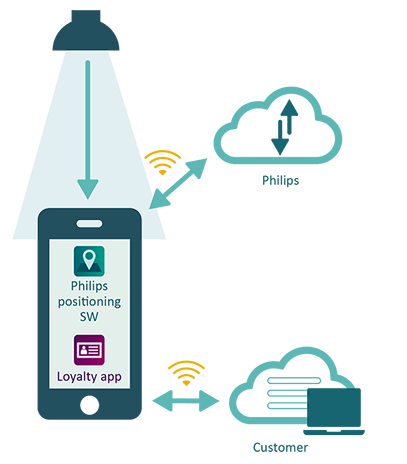
\includegraphics[width=0.5\textwidth]{philips.png}
			\caption{Philips indoor positioning system}
		\end{figure*}

\newpage
\paragraph{}
Disadvantages of the system
	\begin{itemize}
		\item Have to use specially designed LED bulbs with embedded VLC technology
		\item This method is used for promotions which may not be relevant to the customer or choice of the customer since method does not use any analysis information about customer's previous information
		\item No user authentication mechanism is available and any user with the mobile application can use the information
	\end{itemize}

\subsection{INDOO.RS - INDOOR POSITIONING SYSTEM}
This method uses "Trilateration Technique" to pinpoint a location inside a building. Real time data is derived from mix of the following.
	\begin{itemize}
		\item iBeacon Protocol \cite{iBeacons}
			\subitem iBeacon is the name for Apple's technology standard. This allows both Android and iOS devices to listen for signals from beacons and react accordingly. iBeacons allows mobile applications to be aware of its position on a micro-local scale. Bluetooth Low Energy (BLE) technology has been used to communicate between iBeacons and mobile devices.
		\item Senser Fusion
		\item SLAM Engine technology\cite{slam_eng}
	\end{itemize}

\paragraph{}
Disadvantages of the system
\begin{itemize}
	\item Special devices should be used such as iBeacons to locate the position.
	\item This method just provides the location of user and it does not involve in authenticating the user.
	\item Includes additional cost due to special devices required.
	
\end{itemize}


\section{FUNCTIONAL AND NON-FUNCTIONAL REQUIREMENTS}
\subsection{FUNCTIONAL REQUIREMENTS}
\begin{itemize}
	\item Authorized users should be able to connect to the access point only when they are in a position which is allowed by administrator.
	\item Authorized users those who are outside from the allowed area, but have valid user name and password are still not allowed to connect to access point.
\end{itemize}

\subsection{NON-FUNCTIONAL REQUIREMENTS}
\begin{itemize}
	\item Authentication
	\begin{itemize}
		\item Authentication should be done not only with valid user name and password, but also location information according to the Wi-Fi signal strength.
	\end{itemize}
	\item Authorization
	\begin{itemize}
		\item Only authorized parties allow to make modifications, changes to the system.
	\end{itemize}
	\item Availability
	\begin{itemize}
		\item The system should be available in any time whenever user needs to use it.
	\end{itemize}

	\item Reliability
	\begin{itemize}
		\item The system should function without defect under defined conditions/ environment and specific period of time.
	\end{itemize}
	
	\item Usability /User friendliness
	\begin{itemize}
		\item The system should be able to use without extra effort and GUI also need to be easy for the user.
	\end{itemize}
	
	\item Stability
	\begin{itemize}
		\item Application should be stable and all components should function smoothly.
	\end{itemize}
	
\end{itemize}
	
	\chapter{METHODOLOGY}
	\section{INTRODUCTION}
It is known that Wi-Fi access points are vulnerable to remote access of unauthorized users. This research project tries to check the possibility of using location based authentication mechanism for Wi-Fi access point rather than using WPA/ WPA-2 authentication protocols. Location of the user will be measured with respect to user experienced Wi-Fi access point signal strength.

\paragraph{}
This chapter describes techniques related to the research methodology, design of the proposed system and steps that had been carried out to develop the proposed approach. 

\section{BACKGROUND}
\subsection{INVERSE SQUARE LAW}
It can be proven that Wi-Fi access point's signal strength is inversely proportional to the square of distance between device and access point which denotes by the \textbf {Inverse square law} \ref{eq:1}.

\begin{figure}[h]	
	\centering
	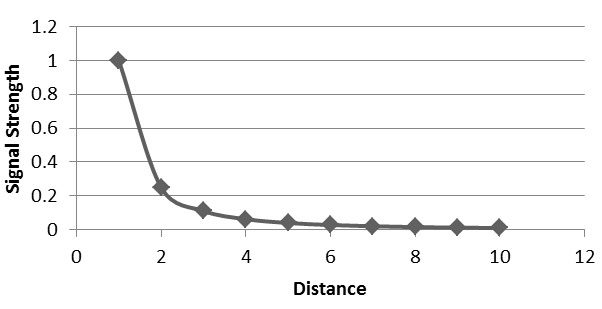
\includegraphics[width=\textwidth]{inverse_square_law.png}
	\caption{Inverse square Law}
\end{figure}

\begin{equation}\boldmath\label{eq:1}
	\beta=\frac{1}{d^2}
\end{equation}\newline


Where:\\
\hspace*{3em}
\begin{tabular}{rl}
	$\beta$:&   received signal strength. \\
	$d$:&  distance between device and access point. \\
\end{tabular}\newline

\paragraph{}
As per the Inverse square law \ref{eq:1}, the received signal strength depends on the distance between user and access point, which means when user goes away from the access point, it results the low received signal strength and wise verse.

\paragraph{}
If the access point is fixed somewhere, it is possible to notice the different level of signal strengths from Wi-Fi access point as per distance.
By using access point's received signal strength, it is possible to identify location uniquely. There are techniques which can be used to identify locations uniquely by using the received signal strength of the Wi-Fi access point.


\subsection{FREE SPACE PATH LOSS}
Since there is a close relationship between received signal strength of the Wi-Fi access point and the distance, distance can be calculated by using following mathematical expression \ref{eq:2}.\newline

	\begin{equation}\boldmath\label{eq:2}
		FSPL(db) = 20\log{10}(d)+20\log{10}(f)+20\log{10}(\frac{4\pi}{c})
	\end{equation}\newline
	
	Where:\\
	\hspace*{3em}
	\begin{tabular}{rl}
		$FSPL(db)$:&   free-space path loss in decibels(received signal strength). \\
		$d$:&  distance between device and access point. \\
		$f$:&  frequency of the access point. \\
		$c$:&  velocity of light in vacuum. \\
	\end{tabular}\newline

\paragraph{}
Free Space Path Loss(FSPL) is defined as \textbf{"The loss between two isotropic radiators in free space, expressed as a power ratio"} \cite{FSPL}
The equation is valid only in an open space(without any obstacles) and here, it cannot be applied directly because the experiment is going to carry out in an environment, which has physical obstacles and also electromagnetic reflection and diffraction.\newline

%\paragraph{}
%The following techniques are used to carry out the project.
\subsection{LOCATION FINGERPRINT TECHNIQUE}

Location fingerprinting technique, which is used to identify each point of the location uniquely according to the RSSI level. In order to fingerprint each point of the desired location, the Wi-Fi access point should be fixed somewhere. Each point's RSSI level changes according to the distance from access point, which makes unique location fingerprint according to the RSSI level. This makes a new location map with respect to RSSI level. Likewise any other maps like Google map uses the combination of latitude and longitude to identify each location uniquely, here the RSSI level will be used to identify the location.

\paragraph{}
This technique requires combination of a radio frequency and map geographical coordinates. The location will be treated as 2-dimension(2D) cartesian plain together with RSSI values.

\paragraph{}
The location fingerprint technique consists of two main phases.
	\begin{enumerate}
		\item Offline training phase
		\subitem Offline survey phase is most important and most critical in this technique. This is a survey of IEEE 802.11 a/b/g/n Wi-Fi signal strength of desired survey area(location which is going to be fingerprint). 
		\paragraph{}
		First, the survey area should be divided into the size of ($1m\times1m = 1m^2$). It is free to decide the area size as per the requirement. But for more accurate survey, more readings are required.
			\begin{figure*}[h]	
				\centering
				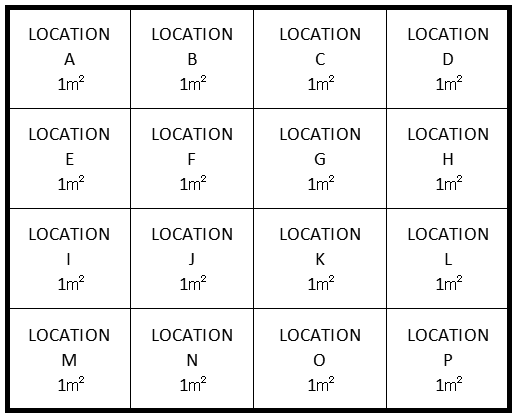
\includegraphics[width=0.5\textwidth]{fp.png}
				\caption{Wi-Fi fingerprinting within area}
			\end{figure*}
		
		Then, the RSSI level of each place should be taken carefully. For more accurate values,the readings(RSSI value) of each location should be taken at least ten(10) times. These readings are stored in a training database which will be used for future assessments of the location.
		
		After this exercise is completed, it is possible to have an average RSSI value of each place. It results a set of data about RSSI level with respect to each location. According to this results, each place can be uniquely identified by using RSSI value for given access point. This is called the location fingerprinting according to the Wi-Fi signal strength.
		
		\begin{description}
			\item NOTE: 
			\subitem Since Wi-Fi signal strength relates with the distance as per the equation \ref{eq:1}, the Access point should be fixed permanently. If the Access point location is changed or Access point hardware is changed, the process should be done from the beginning and training database should be populated with fresh RSSI information. 
		\end{description}
		
		\item Online positioning phase
		\subitem This is where the previous training database is in use. Pointing the user's location by comparing real time data with the information that had been captured in previous phase (known as training database). If offline training phase was completed successfully, online positioning phase can be done quiet easily with more accurate results.
		
		\subitem 
		Wi-Fi signal information (RSSI values) should be captured at real time and it has to be passed to  the place where the position is going to be calculated(server). This server uses the training database and compares the provided Wi-Fi signal strengths with training database data. From that, it can be detected the user's location with respect to Wi-Fi signal strength.
	\end{enumerate}


\subsection{TRILATERATION TECHNIQUE}
The process of calculating the position of the object by using a mathematical way is called "Trilateration".\cite{trilateration} Suppose there are three signal generators A,B,C located in a cartessian plain and each signal generator can fully cover the whole area by itself. 

		\begin{figure*}[h]	
			\centering
			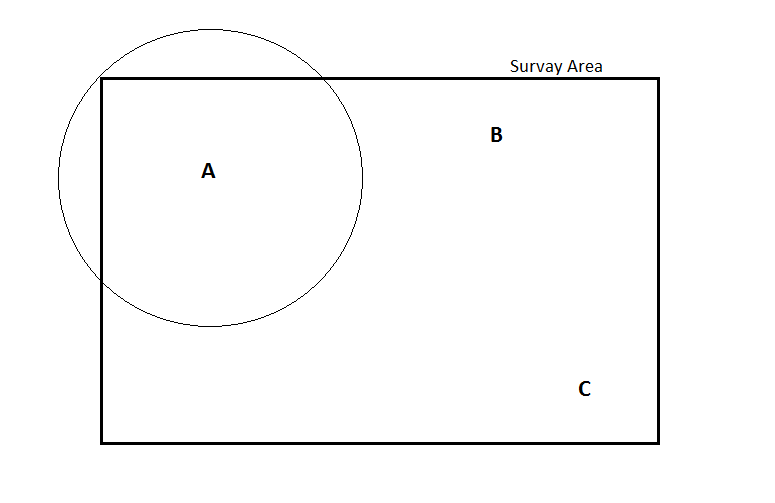
\includegraphics[width=0.8\textwidth]{tri_1.png}
			\caption{Trilateration - Signal Generator A's coverage }
		\end{figure*}

Signal generator(A) generates a signal with specific time and distance and broadcasts that particular signal over air. Even though this signal hits the receiver by any angle, it provides the distance. So this distance forms a circle with a radius of itself. Which means the receiver's location could be anywhere on this circle. Likewise the second signal generator(B)'s signal is also received by the receiver.

\begin{figure*}[h]	
	\centering
	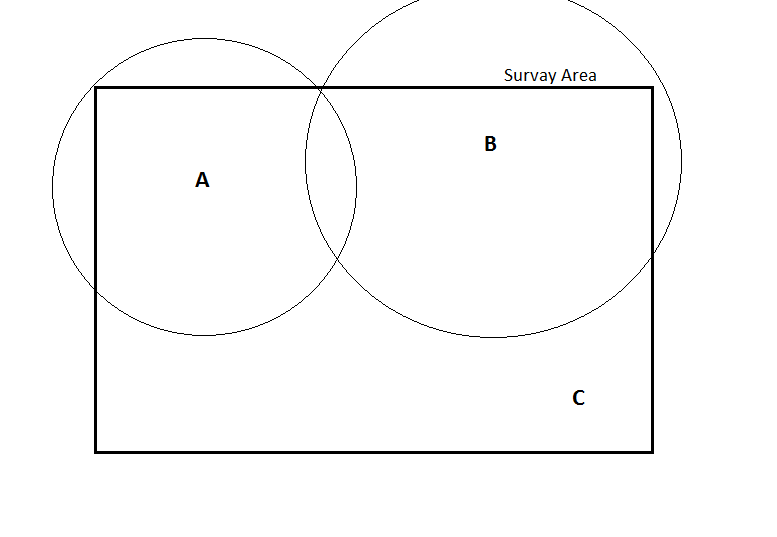
\includegraphics[width=0.8\textwidth]{tri_2.png}
	\caption{Trilateration - Signal Generator B's signal received }
\end{figure*}

This distance is also equally broadcast in all directions. By this time, the receiver has two known distances from two signal generators. The precise position could be at any of the two positions where two circles intersect. With the third signal generator(C), it reveals true location of the receiver where all three circles intersect.

\begin{figure*}[h]	
	\centering
	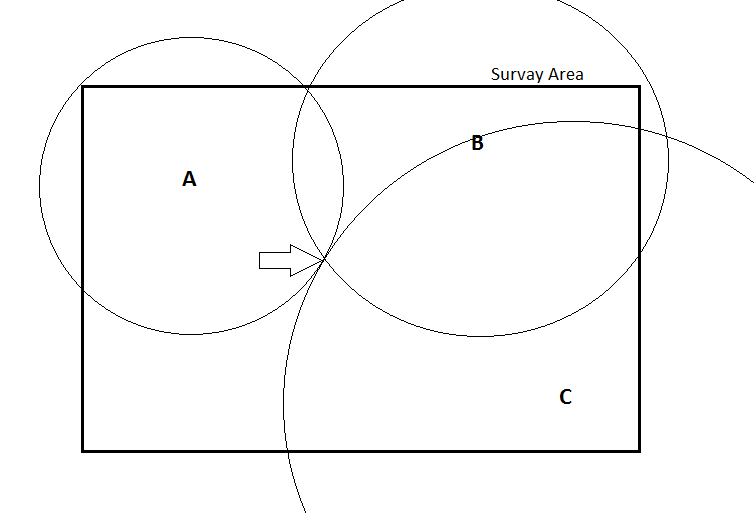
\includegraphics[width=0.8\textwidth]{tri_3.png}
	\caption{Trilateration - Receiver's location }
\end{figure*}

\paragraph{}
There are two types of trilateration techniques available.\cite{trilateration_2}
\begin{enumerate}
	\item 2-D Trilateration
		\subitem In this technique it uses two-dimension(2-D) cartesian plain to locate receiver. The signal generators broadcast their signals in a circular manner. 

	\item 3-D Trilateration
		\subitem In this technique, it uses three-dimension(3-D) cartesian plane to locate receiver. Likewise 2-D trilateration, 3-D trilateration broadcasts its signal in spherical manner.
\end{enumerate}

\paragraph{}
 Trilateration method is being used practically by Global Positioning Service (GPS) satellites to locate users. These satellites broadcast signals in a spherical manner (3-D trilateration) and where all spheres intersect determines the position of the GPS receiver. 
 
 \newpage
 \subsection{HYBRID TECHNIQUE}
 Combination of LOCATION FINGERPRINT TECHNIQUE and TRILATERATION TECHNIQUE is called HYBRID TECHNIQUE.\cite{hybrid_tech} Location fingerprinting technique can fingerprint each location uniquely with respect to Wi-Fi signal strength. By using Trilateration technique, it is possible to locate receiver(user)'s location even inside in a building. With the combination of those two techniques, the receiver's location can be retrieved without using any other locational technique such as GPS. 
 
 \subsection{RADIUS PROTOCOL}
 Remote Authentication Dial-In User Service (RADIUS) is an industrial standard for distributed remote access networking which provides authorization, authentication, accounting and identification.\cite{radius_protocol} Protocol uses Password Authentication Protocol(PAP), Challenge Handshake Protocol(CHAP), Extensible Authentication Protocol(EAP) to authenticate users. RADIUS can look text file,Database or LDAP server for authentication.
 
 \paragraph{}
 The RADIUS server consists of three main authentication responses.
 
 	\begin{itemize}
 		\item Access Accept
 			\subitem Once the user is authenticated, the RADIUS server returns this response. Then the server will often check whether user is authorized or not, to use network. 
 		\item Access Challenge
 			\subitem This requests additional information by server such as PIN, token or secondary password to authenticate the user.
 		\item Access Reject
 			\subitem User is denied to access to all requested network access due to the authentication failure.
 	\end{itemize}
 
 \begin{figure*}[h]	
 	\centering
 	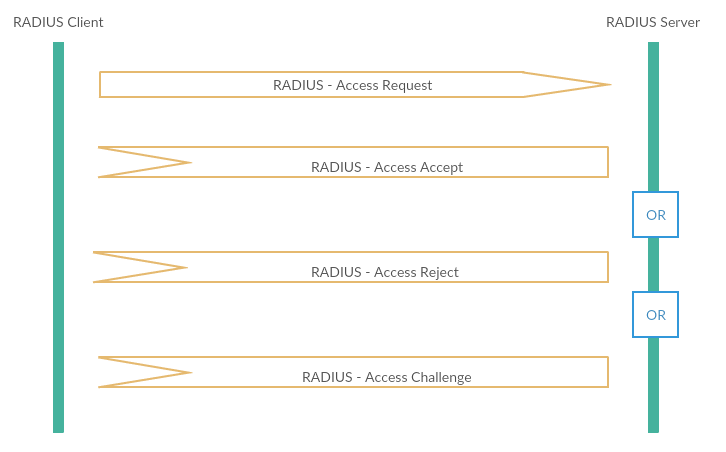
\includegraphics[width=0.8\textwidth]{radius_auth.png}
 	\caption{RADIUS authentication process}
 \end{figure*}
 
 RADIUS client can be any user, who is requesting access from RADIUS server. First user sends Access-Request to the RADIUS server together with user credential information and server checks whether user is valid or not. According to the validation, the server sends appropriate response as per the protocol that server is using for.
 
 \paragraph{}
 For this research project, "FreeRADIUS SERVER" has been used as the RADIUS server.
 
 \paragraph{}
 \begin{center}
 	\begin{table}[H]			
 		\begin{tabu}  { | X[c] | X[c] | }	
 			\hline
 			FreeRADIUS Strengths& FreeRADIUS Weakness \\
 			\hline
 			\begin{itemize}
 				\item Open source
 					\subitem FreeRADIUS is releasd under general public licence. It is free to use, change and whatever fix as required.
 				\item Availability
 					\subitem Supports to all popular Linux distribution and also for Windows operating system.
 				\item Active development
 					\subitem Since FreeRADIUS is an open source and it has world wide development community, FreeRADIUS is being rapidly updated.
 				\item Powerful
 					\subitem FreeRADIUS is capable of supporting file based authentication and  database based authentication.
 				\item Used by mass
 					\subitem Large organizations also use FreeRADIUS not only in sri lanka, but also all around the world.
 			\end{itemize} & 
 			\begin{itemize}
 				\item Complexity
 					\subitem FreeRADIUS offers an all-inclusive piece of software with many configuration options. If any of the configuration is missed or incorrectly configured, it ends up with broken system.
 				\item Vulnerabilities
 					\subitem Few vulnerabilities have been published.
 			\end{itemize}\\
 			\hline
 		\end{tabu}
 		\caption[FreeRADIUS strengths and weaknesses]{FreeRADIUS strengths and weaknesses}
 		\label{table:aimPt_isol}
 	\end{table}
 \end{center} 
 
 
 \subsection{ANDROID WifiEnterpriseConfig API}
 Android WifiEnterpriseConfig application programming interface(API) supports the RADIUS protocol\cite{wpa2_enterprise} from API level 18 and above. For the android mobile application, this API is used to communicate between FreeRADIUS server and user.
 
\section{STEPS FOLLOWED}

\paragraph{}
In this research, HYBRID TECHNIQUE has been used to locate receiver(user)'s location. FreeRADIUS server has been used as authentication server. MySQL is used as relational database. Android WifiEnterpriseConfig API integrated application has been used as Wi-Fi connector. Ubuntu 14.04 server is used as host server. This research process has been done through a series of steps and with phases. The steps that have been carried out throughout the research are as follows.

	\begin{enumerate}
		\item Setup FreeRADIUS server for Wi-Fi user authentication.
		\subitem Reasons for the choice of FreeRADIUS are,
		
		\begin{enumerate}
			\item FreeRADIUS is powerful and allow more customization in configurations.
			\item It is free to use and free to modify.
			\item Capable of supporting PHP server side scripting and MySQL database for the Wi-Fi authentication process.
			\item Supports Ubuntu distribution.					
		\end{enumerate}
			\subitem FreeRADIUS server has been installed to Ubuntu 14.04 virtual host server with PHP and MySQL services. FreeRADIUS server configuration has been modified to execute PHP script and PHP script has been designed to access training database. 
		
		\item Use Wi-Fi enterprise support access point as main Wi-Fi access point. 
			\subitem Normal home use Wi-Fi access points are not supported to RADIUS protocol. in order to support RADIUS protocol, the device should be able to support Wi-Fi enterprise techniques. From the configuration of the access point, it should be possible to configure to redirect the authentication requests from users to the RADIUS server by providing server's IP address and pre-shared secret. When user authentication request is received, the access point does not try to authenticate the user, but the access point redirects the authentication traffic to RADIUS server. The RADIUS server is responsible to authenticate users and provide appropriate response back to the user.
	
		\item Build Android mobile application with WifiEnterpriseConfig API to provide a required data to authenticate Wi-Fi user via FreeRADIUS server. 	
			\subitem This application is supported by providing information for both off-line training phase of location fingerprinting technique and on-line positioning phase. The provided data from the android mobile device to the authentication server would be RSSI values of each Wi-Fi access point, access point specific data, user name, password. All data are in a single Java Script Object Notation(JSON) object and this JSON object is passed to the authentication server via Wi-Fi access point.
		
		\item Fix three(03) Wi-Fi access points together with enterprise support access point to cover entire research area by each, in different locations. 
		\subitem Wi-Fi trilateration technique requires three access points for the location measurement. And with more number of access points, it can take more accurate fingerprint data for a location.
		
		\item Collect selected location data by using developed android mobile application and populate training database with collected location data within RADIUS server.
		\subitem Developed android mobile application consists of training mode. By enabling the training mode, the server can store the Wi-Fi signal data inside the training database. 
		
		\item Analyze collected data from training database and calculate maximum and minimum Wi-Fi RSSI values for each location for each access point and create a new table with extracted data.  
		
		\item Integrate Wi-Fi location fingerprint database with RADIUS server and use the fingerprint database together with user name and password for Wi-Fi user authentication.
		
		\item On-line location analysis process uses training database to authenticate users
		
		\item Analyze results for conclusion.
		
		\item Develop a back end web based application to control Wi-Fi users.
	\end{enumerate}
 
 
 
 

 
	
	\chapter{DESIGN}
	\section{INTRODUCTION}
System design has been carried out by using several software engineering techniques and some of the design methods and design diagrams are discussed in this chapter. The diagrams are designed according to the gathered requirements.

\section{DESIGN DIAGRAMS}
\subsection{TOP LEVEL NETWORK DIAGRAM}
\begin{figure}[H]	
	\centering
	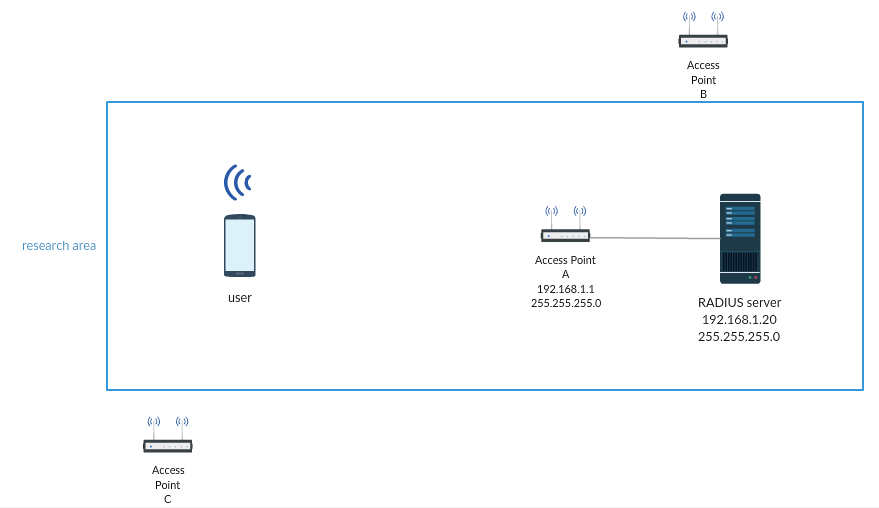
\includegraphics[width=0.9\textwidth]{toplevel_3.png}
	\caption{Top Level network Diagram}
\end{figure}

Three Wi-Fi access points (A,B and C) are fixed in three separate places and the access point A, which is enterprise support access point is connected to the RADIUS server by directly via network cable. 


\subsection{DATABASE DIAGRAM}
Proposed approach does not use complex database to authenticate users. Three main non-relational tables are being used to authenticate users.

\paragraph{}
Database design is carried out by using standard database normalization methods and there are two databases designed for the local database and the central database. Since the proposed solution uses RADIUS server for Wi-Fi user authentication, the MySQL database is running with authentication server to store all necessary data for user authentication.

\paragraph{}
within the Android application, data has been stored as shared preferences which contains user location information with respect to time.

\begin{figure}[h]	
	\centering
	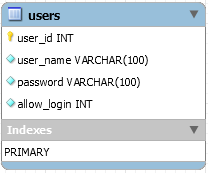
\includegraphics[width=0.3\textwidth]{users_table.png}
	\caption{Users table}
\end{figure}

\newpage
\paragraph{}
Users table contains all user information together with user name, password and special flag "allow login" to control user access by an administrator. This table is used by RADIUS server and also back end administration panel to manage user logins. 

\begin{figure}[h]	
	\centering
	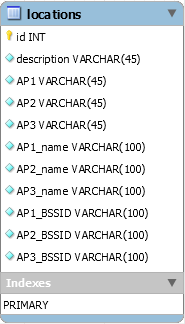
\includegraphics[width=0.3\textwidth]{locations_table.png}
	\caption{Location table}
\end{figure}
\paragraph{}
Location table is the place where all the data that has been collected by off-line training phase of the location fingerprinting technique is initially stored. This table contains all raw data of the Wi-Fi signal strengths (RSSI value) of each location of the research area. 

\begin{figure}[h]	
	\centering
	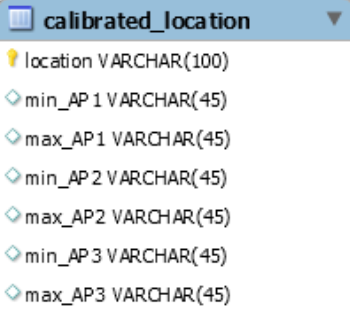
\includegraphics[width=0.3\textwidth]{calibrated_table.png}
	\caption{Calibrated location table}
\end{figure}

\newpage
\paragraph{}
This table view is generated by analyzing the location data table and retrieving the maximum and minimum RSSI value for each location for each Wi-Fi access point. This is the most important data source that is being used to authenticate user in on-line authentication phase of the location fingerprinting technique.

\subsection{ACTIVITY DIAGRAM}

\begin{figure}[h]	
	\centering
	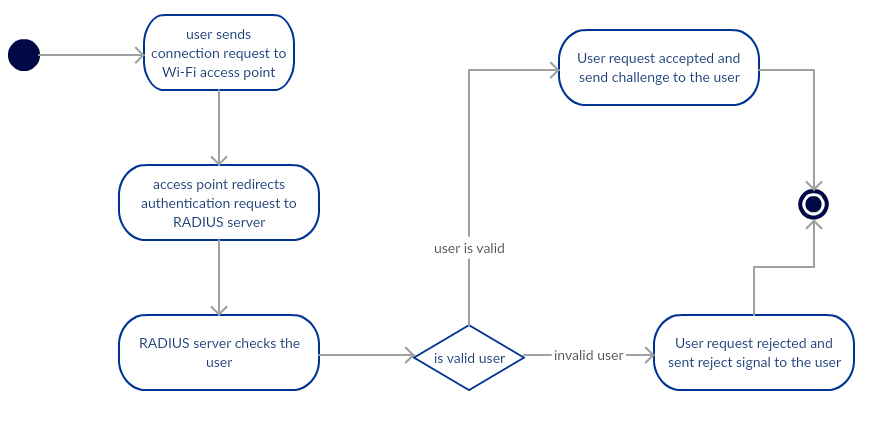
\includegraphics[width=1\textwidth]{activity_diagram.png}
	\caption{Activity diagram}
\end{figure}

\paragraph{}
Overall activity of the process is shown in activity diagram. This provides the general idea of the process. 

\newpage
\subsection{SYSTEM DESIGN}
Wi-Fi signal strength of each location of the identified area should be measured by using Wi-Fi signal strength measuring tool.
Since we know the exact location of the access point, we can measure the distance from each access point to pointed location.

\begin{figure}[h]	
	\centering
	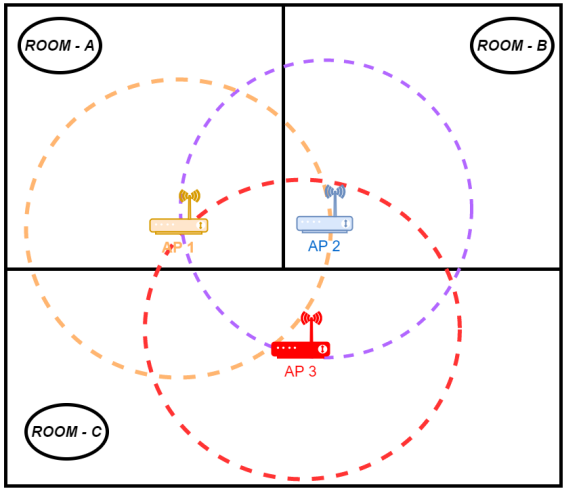
\includegraphics[width=0.8\textwidth]{signal_distribution.png}
	\caption{Signal Distribution of Wi-Fi access points}
\end{figure}

%\subsection{DATABASE DESIGN}

	
	\chapter{IMPLEMENTATION}
	\section{INTRODUCTION}
This chapter describes the implementation of the proposed system, step by step. Since the research has been carried out by few implementation phases, those implementation phases are described as follows. 

\section{SETUP FreeRADIUS SERVER}
Ubuntu 14.04 has been taken as the host server implementation. All server implementations have been done on top of Ubuntu operating system.

\paragraph{}
\begin{center}
	\begin{figure*}[h]	
		\centering
		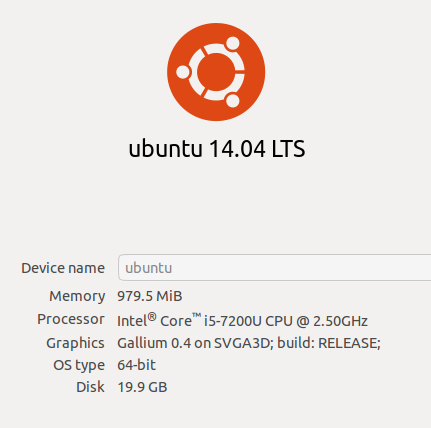
\includegraphics[width=0.4\textwidth]{ubuntu.png}
		\caption{Host server specification}
	\end{figure*}
\end{center} 

\subparagraph{NOTE : }
The host server should have root access for the implementation.

\paragraph{}
 \begin{itemize}
 	\item Install FreeRADIUS services, MySQL, PHP and other required modules\cite{freeradius}. 
 	\begin{lstlisting}
	apt-get install freeradius php-common 
	php-gd php-curl php-mail php-mail-mime 
	php-pear php-db php-mysql freeradius-mysql 
 	\end{lstlisting}
 		
 	\item Edit \verb |\etc\freeradius\clients.conf | to accept and communicate with Wi-Fi access point (IP 192.168.1.1/255.255.255.0) by adding following code snippet at the end of the file.
 	\begin{lstlisting}
 	client LBA_AP{
 	ipaddr	= 192.168.1.1
 	secret	= testing123
 	 }
 	\end{lstlisting}
 		
 		The "ipaddr" is the IP address of the Wi-Fi access point and the "secret" is the pre-shared key between RADIUS server and Wi-Fi access point. The client name is defined as \verb|"LBA_AP"|.
 		
 	\item It is known that the RADIUS protocol uses port 1812 and port 1813 for its operations. Therefore by executing following commands, allow access to the relevant ports from Ubuntu firewall.
 	\begin{lstlisting}
	ufw allow 1812
	ufw allow 1813
 	\end{lstlisting}
 		
 		
 	\item Since the technique uses MySQL database, the database has to be created and populated the tables as per the data. To create new database "lba" and create tables,
 	%\begin{appendices}
 	
 	\begin{lstlisting}
 	create database lba;

 	create table users 
 	(user_id int primarykey auto_increment,
 	user_name varchar(100) not null,
 	password varchar(100) not null,
 	allow_login int default 1);
 		
 	create table locations 
 	(id int primarykey auto_increment,
 	description varchar(45) not null,
 	AP1  varchar(45) not null,
 	AP2  varchar(45) not null,
 	AP3  varchar(45) not null,
 	AP1_name  varchar(100) not null,
 	AP2_name  varchar(100) not null,
 	AP3_name  varchar(100) not null,
 	AP1_BSSID  varchar(100) not null,
 	AP2_BSSID  varchar(100) not null,
 	AP3_BSSID  varchar(100) not null);
 		
	 create or replace view calibrated_locations as
	 select description as location,
	 min(AP1) as min_ap1,
	 max(AP1) as max_ap1,
	 min(AP2) as min_ap2,
	 max(AP2) as max_ap2,
	 min(AP3) as min_ap3,
	 max(AP3) as max_ap3 
	 from locations 
	 group by description
	 order by description asc;
 	\end{lstlisting}
 	%\end{appendices}
 		\item After creating tables, the FreeRADIUS server was configured to use the created database through PHP script. Refer authscript.php from appendix \ref{php_script}
 		
 			\subitem this PHP script handles both populating off-line training database and on-line positioning phase of the location fingerprinting technique. The following code snippet directs RADIUS server to execute PHP script.\cite{freeradius_2}
 			
 			Edited \verb|/etc/freeradius/sites-enabled/default| file and added the code at the end of the block \verb|authorize {}|\cite{freeradius_php}
 			
 		\begin{lstlisting}
 		update control {
 		Auth-Type := `/usr/bin/php -f
 		/etc/freeradius/authscript.php 
 		'%{User-Name}' 
 		'%{User-Password}' 
 		'%{Client-IP-Address}'`
 			}
 		\end{lstlisting} 
 	
 		\subitem Now FreeRADIUS server is ready and restarted by using following commands.
 		\begin{lstlisting}
 		/etc/init.d/freeradius stop
 		/etc/init.d/freeradius start
 		\end{lstlisting}
 \end{itemize}

\newpage
\section{SETUP WI-FI ROUTER}
The Wi-Fi router has been configured to forward all authentication requests to the FreeRADIUS server. The used Wi-Fi router is DCP LINK ,model "DCP-WR300N".

%\paragraph{}
\begin{center}
	\begin{figure*}[h]	
		\centering
		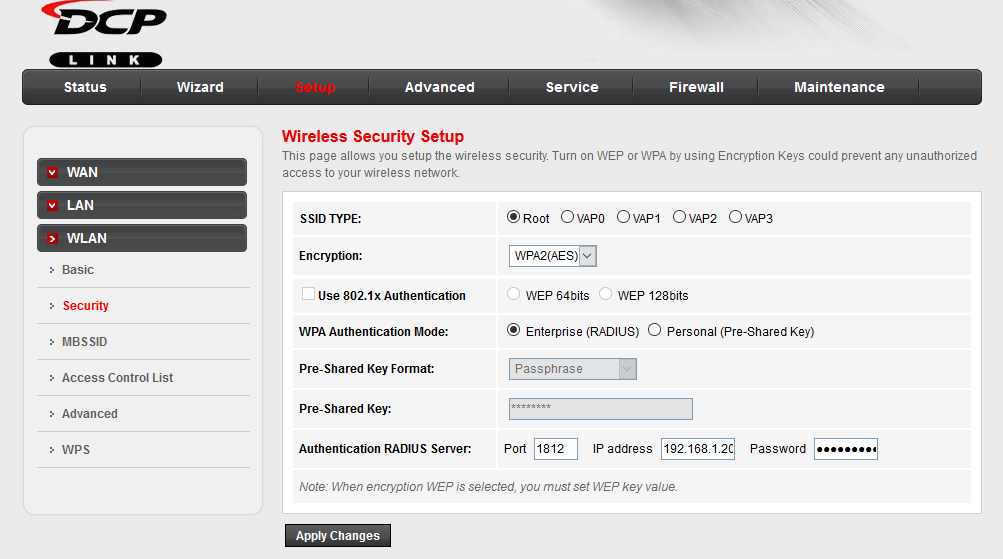
\includegraphics[width=1\textwidth]{router_config.png}
		\caption{Wi-Fi router configuration}
	\end{figure*}
\end{center} 

Router configured for WPA2(AES) encryption and WPA Authentication mode set to Enterprise(RADIUS). Authentication RADIUS server port has configured as 1812, IP address as 192.168.1.20/255.255.255.0 and the most important pre-shared secret is set as per the FreeRADIUS server's \verb|\etc\freeradius\clients.conf| file. It is pretty straight forward and easy to configure Wi-Fi router to authenticate via FreeRADIUS server. FreeRADIUS server and W-Fi router are connected by using wired connection.

\section{DEVELOP ANDROID MOBILE APPLICATION}
The Android mobile application is the tool that used to collect Wi-Fi signal strength of each location with respect to each access point. User has to nominate three(03) access  points from available access points list which are provided in the application settings menu, by scanning Wi-Fi access points in real time, for the authentication process.

\begin{center}
	\begin{figure*}[h]	
		\centering
		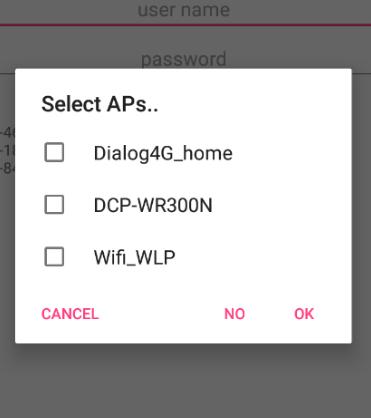
\includegraphics[width=0.5\textwidth]{select_ap.png}
		\caption{Select Access Points first}
	\end{figure*}
\end{center}

\newpage
This selected three(03) access points information will be collected by the application and make a JSON object to send to the authentication server. Sample JSON object is as follows.\cite{jsonlint}
	\begin{lstlisting}
	{
		"name": "username",
		"password": "userpassword",
		"ap3name": "AP3_name",
		"ap3": -69,
		"ap3_BSSID": "c8:b5:ad:8b:dd:a0",
		"ap2name": "AP2_name",
		"ap2": -72,
		"ap2_BSSID": "08:5b:0e:10:2b:0a",
		"ap1name": "AP1_name",
		"ap1": -79,
		"ap1_BSSID": "2a:5b:0e:0f:e6:aa",
		"desc": "",
		"save": "n"
	}
	
	\end{lstlisting}

\newpage
Method wpa2enterprise() stands for providing necessary information to the FreeRADIUS server to authenticate user. \cite{wifi_connect}
Refer appendix \ref{android_api} for wpa2enterprise() method.

\begin{center}
	\begin{figure*}[h]	
		\centering
		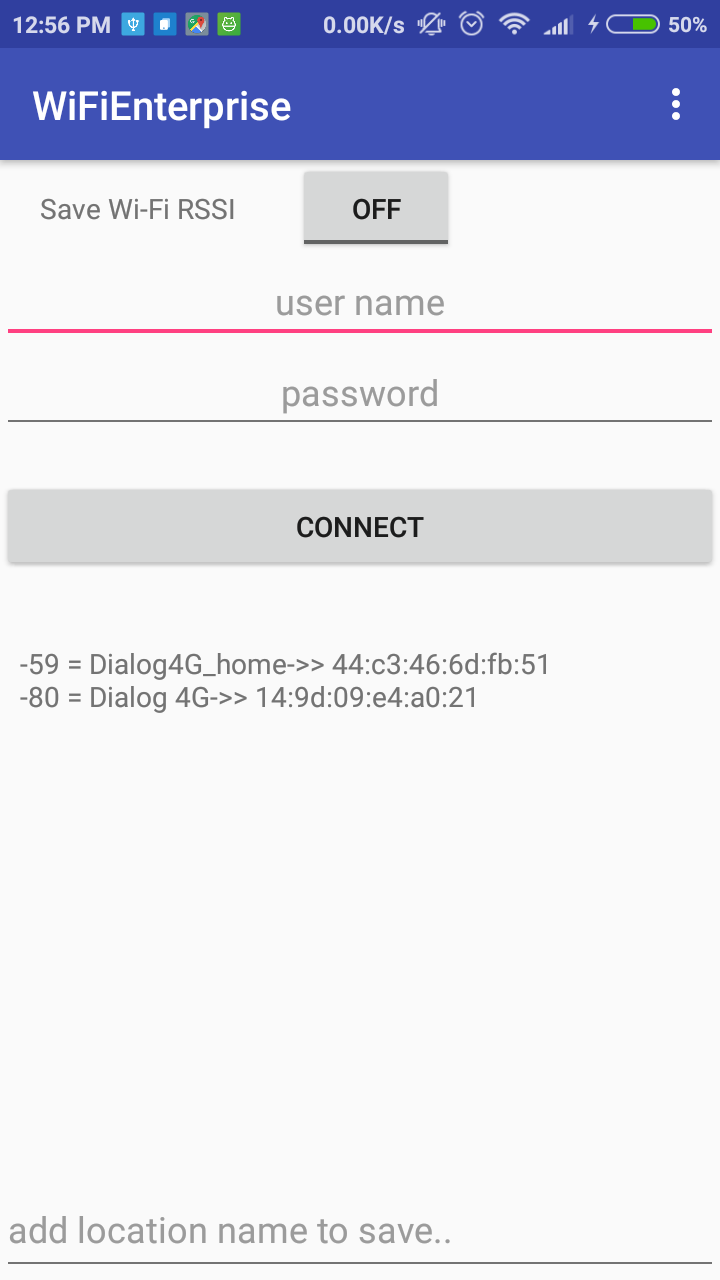
\includegraphics[width=0.4\textwidth]{mobile_app.png}
		\caption{Android Mobile Application}
	\end{figure*}
\end{center}

\newpage
\section{DEVELOP BACK END ADMINISTRATION PANEL}
Back end administration panel is web based back end application which supports to the administrator to control Wi-Fi users such as add new user, allow and deny access to the existing users.  

\begin{center}
	\begin{figure*}[h]	
		\centering
		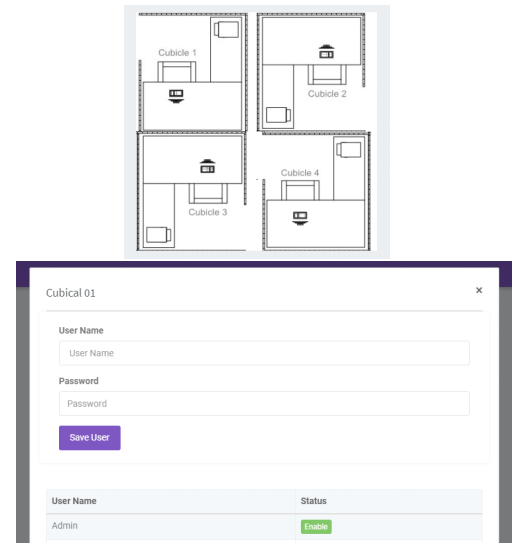
\includegraphics[width=0.6\textwidth]{backend.png}
		\caption{Back end admin panel}
	\end{figure*}
\end{center}

\newpage
\section{FREERADIUS STATIC TESTING TOOL}
NTRPing is a useful tool for testing installation of the RADIUS server. By using this tool, it is possible to simulate authentication and accounting requests and send them to the RADIUS server. 

\begin{center}
	\begin{figure*}[h]	
		\centering
		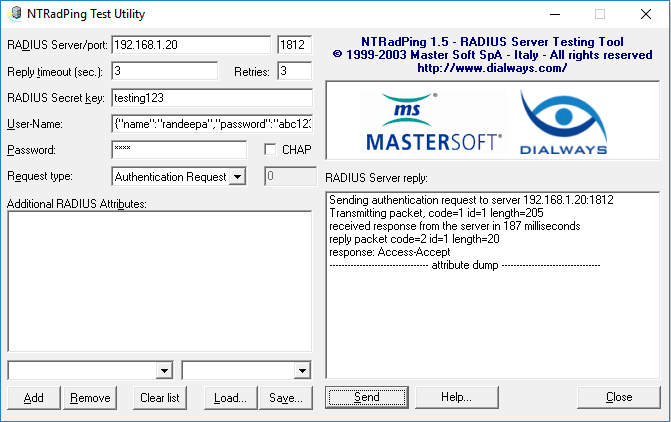
\includegraphics[width=0.8\textwidth]{ntrping.png}
		\caption{NTRPing tool}
	\end{figure*}
\end{center}

It is easy to check the RADIUS server by using this tool since NTRPing tool is acting like NAS client.\cite{ntrping_tool}

%\section{LOCATION FINGERPRINT DATA}
	
	\chapter{EVALUATION}
	\section{INTRODUCTION}
This chapter describes the collected data and analysis of the data. Expected results and actual results are discussed here and the deviation of the actual results from expected results are shown. The improvements that could be done  to minimize deviation from the expected is also discussed within this chapter. Further improvements that can be done for the research and how those improvements can be done are also discussed.

\section{ANALYSIS OF DATA}
Data collection has been done for 07 times per location (selected $1m^2$ area)to collect Wi-Fi RSSI values for each location by using developed android application. Each collected data has been analyzed separately and finally all data had been analyzed with respect to each location. The data analyzation will be discussed here after.

\newpage
\subsection{ACCESS POINT 01 DATA ANALYSIS}  
\begin{center}
	\begin{figure*}[h]	
		\centering
		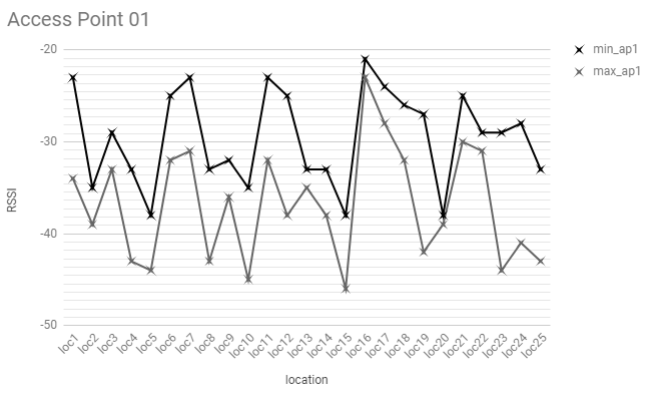
\includegraphics[width=1\textwidth]{ap1.png}
		\caption{Access Point 01 data analysis}
	\end{figure*}
\end{center} 

This line chart shows the Wi-Fi RSSI range of access point 01 (Wi-Fi enterprise support access point which directly communicates with FreeRADIUS server). There are two graphs in the chart which clearly shows minimum RSSI values of each location and maximum RSSI value of each location. It can be identified that the difference between maximum and minimum RSSI value of each location is around 10 dB's.

\newpage
\subsection{ACCESS POINT 02 DATA ANALYSIS}  
\begin{center}
	\begin{figure*}[h]	
		\centering
		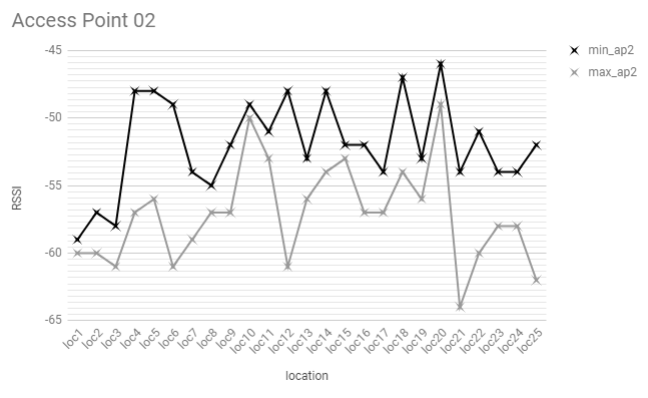
\includegraphics[width=1\textwidth]{ap2.png}
		\caption{Access Point 02 data analysis}
	\end{figure*}
\end{center} 

This line chart shows the Wi-Fi RSSI range of access point 02. There are two graphs in the chart which clearly shows minimum RSSI values of each location and maximum RSSI value of each location. Not like the previous access point, this access point is located outside the research area which has physical obstacles. It seems that the signal strength of this access point is fluctuate significantly.

\newpage
\subsection{ACCESS POINT 03 DATA ANALYSIS}  
\begin{center}
	\begin{figure*}[h]	
		\centering
		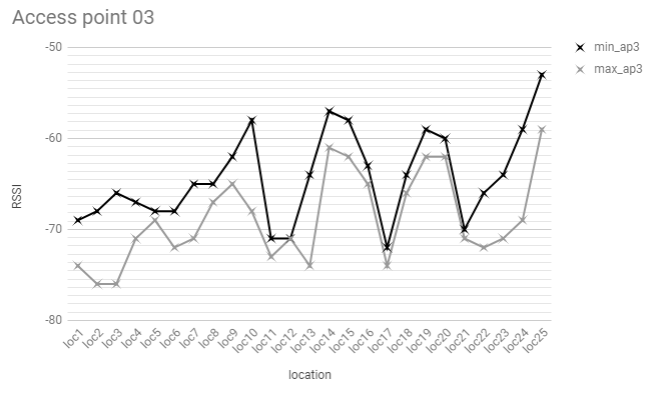
\includegraphics[width=1\textwidth]{ap3.png}
		\caption{Access Point 03 data analysis}
	\end{figure*}
\end{center} 

This line chart shows the Wi-Fi RSSI range of access point 03. There are two graphs in the chart which clearly shows minimum RSSI values of each location and maximum RSSI value of each location. This access point is also located outside the research area which has physical obstacles. But as an average, this access point is far away from the research area. Therefore, the signal strength of this access point is much weaker than the previous two access points.

\newpage 
\subsection{ALL ACCESS POINT DATA ANALYSIS}  
\begin{center}
	\begin{figure*}[h]	
		\centering
		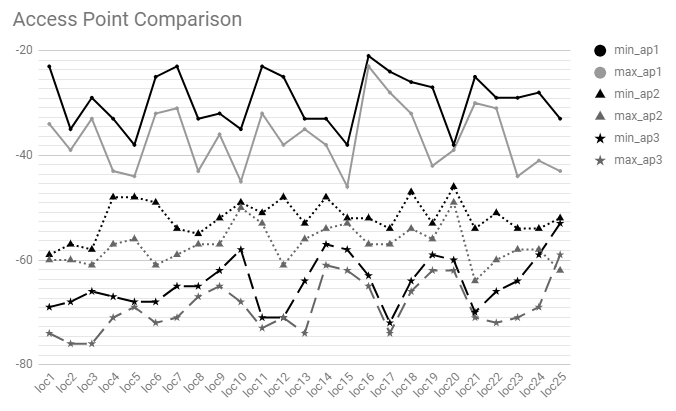
\includegraphics[width=1\textwidth]{total_comparison.png}
		\caption{Access Point data analysis}
	\end{figure*}
\end{center} 

All three(03) access point RSSI values are compared here. Each access point is marked by a separate symbol.

\newpage
\subsection{LIVE USER ACCESS DATA ANALYSIS}

In this phase, user live access data has been collected for the access attempts of 140. 125 readings have been taken within the research area where the location fingerprinting has been done. The rest of the readings were taken by accessing the system from outside of the research area. The testing of the system has been carried out with uncontrollable noisy of additional Wi-Fi signals.

\begin{figure*}[h]
	\centering
	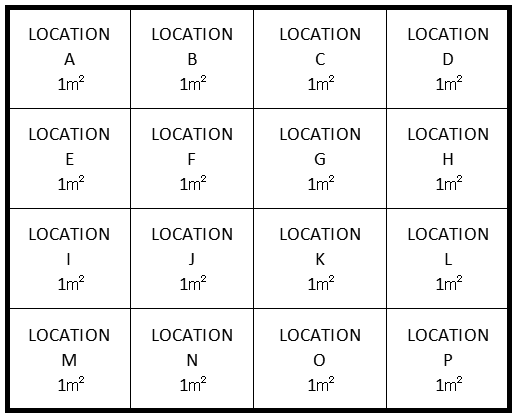
\includegraphics[width=0.4\textwidth]{fp.png}
	\caption{Wi-Fi fingerprinting area}
\end{figure*}
Refer appendix \ref{LOCATION ONE TEST} for each location test results.

\paragraph{}
By analyzing the test results, it is possible to identify that some location results are significantly deviated from the expected results. There could be several reasons for the deviation.

\subsubsection{OVERALL TEST RESULT}
\begin{table}[H]
	\centering
	\label{OVERALL TEST RESULT}
	\begin{tabular}{lllll}
		NO OF LOCATIONS& :&  25&    \\
		SUM OF PASS RATE& :& 1980&  \\
		SUM OF FAIL RATE& :& 520&   \\\\
		AVERAGE PASS RATE& :& $\frac{1980}{25}$&   \\\\
		AVERAGE FAIL RATE& :& $\frac{520}{25}$&  \\\\
		OVERALL PASS RATE& :& \verb|79.20%|&   
	\end{tabular}
	\caption{Overall Test Results}
\end{table} 


\section{FACTORS EFFECTING TO WIRELESS NETWORK SIGNAL}
It is well known that wireless networks use electromagnetic waves(radio waves) for the communication. Even though electromagnetic waves do not require any medium for propagation, there are many factors that could be affected to the performance of the Wi-Fi network. Some of those cannot be avoided and measures have to be taken to minimize the negative effects which are affecting on the performance. The rest of the factors can be completely resolved by either through a good network planning or equipment upgrading.\cite{signal_probs}
\begin{itemize}
	\item Network range and distance between devices
	
	\begin{figure*}[h]	
		\centering
		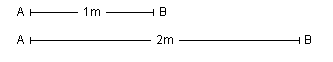
\includegraphics[width=0.4\textwidth]{distance.png}
		\caption{Signal strength with distance}
	\end{figure*}
	
	\subitem  Due to the wireless signal propagation within wide areas when they travel further, the signals become weaker. Inverse Square Law \eqref{eq:1} denotes this relationship between signal strength and the distance.
	
	\item Physical interference
	\subitem There is a possibility of penetrating Wi-Fi signals through solid objects such as buildings, walls, hills or even people. The more obstacles between signal generator and receiver, the more impact on signal strength. With lower frequency of the signal, there is a high impact on the signal strength. And also with higher frequency, the reflection capabilities get increased. However in some cases, reflecting may work better rather than trying to send it directly.
	
	\item Network usage
	\subitem Wireless networks allow more than one user to communicate over the channel simultaneously. That means the network resources are utilized by many users and when more devices are connected to the access point, it easily comes to the threshold level and this makes a reduction in performance.
	
	\item Wireless network interference
	\subitem Since wireless networks are common, more wireless transmissions are being sent through the open air and those signals could be operated at similar frequencies. It is well known and proved that the waves operating at similar frequencies can cause an interference with each other and the resultant signal may completely different from the generated signal. Other wireless technologies such as microwave, mobile phone signals that operate within the same range could be affected to the signals as well. But most of the devices are designed to minimize such effects as much as possible by the design, but still the effects are present with an acceptable level.
	
	\item Environmental characteristics
	\subitem Physically,concrete wall obstacles are the biggest constraint of wireless signals. The materials used in the walls may have different levels of effects as well. And also the humidity in air also effects the signal strength, negatively. The moisture in the air makes it more difficult for the signal to be sent efficiently.\cite{humidity_issue} Other than that, any object which is located between signal transmitter and receiver can absorb some sort of energy of the signal, which may result a negative impact on the signal strength within the area.
\end{itemize}  


\section{FURTHER IMPROVEMENTS}
The suggested approach is expected to pass more than \verb|90%| test cases but the actual pass rate of the total test cases is less than expected rate. Because of this, more improvements are required to gain the pass rate of test cases as expected.

\begin{itemize}
	\item Collect more location data to improve accuracy of the location fingerprint database
		\subitem The research has been carried out with seven(07) rounds of data collection sets. More collected location data can minimize the Wi-Fi RSSI value reading errors.
		
	\item Collect data with different conditions.
		\subitem Data can be collected in both calm and noisy environmental conditions. But collecting data should be done carefully as noisy and bad environmental conditions can badly affect to the Wi-Fi RSSI values, Which may result in accepting users those who are coming from the outside of the allowed location.
		
	\item Harden the RADIUS server to avoid possible vulnerabilities.
		\subitem The system completely depends on location fingerprint database. Therefore separate, dedicated user should be used for RADIUS server rather than super user.
		
	\item Encrypt data objects from Android mobile application to RADIUS server.
		\subitem Data object (JSON object) is a plain text format. It could be vulnerable for sniffing attacks. It should use a proper encryption method to encrypt data.
		
	\item Add a separate database user for MySQL database (Location fingerprint database).
		\subitem It is better to use a separate user for database transactions rather than using super user with a complex password. This separate user should be able to perform only the following operations.
			\subsubitem Read data
			\subsubitem Write data
			\subsubitem Update data
		 
	\item Build self-learned location fingerprint database
		\subitem Collect data of the Wi-Fi signal strengths at real time by using android application to build self-learned Wi-Fi fingerprint database. Authentication failures could be minimized by this such as mistakes of initial training database errors.
		
	\item Minimize human errors when collecting initial data collection
		\subitem Human errors are common in most of the systems and it is difficult to minimize. The same person could be used to collect data, to minimize human errors which can be happened when collecting initial Wi-Fi signal data.
\end{itemize}
	
	\chapter{CONCLUSION}
	\section{OVERVIEW}
Technology has become one of the key factors in business and it plays a critical role in most of the organizations. Introduction of Wi-Fi technology has terminated the wired networking problems and has introduced a mobility networking approach. Along with these advantages of Wi-Fi technology, there are hidden drawbacks like in other technologies. In order to mitigate or reduce those drawbacks, scientists and professionals are still trying for new methods. Wi-Fi technology, is used in many places to carry out really critical functional operations in the business or organization, so as hackers tend to discover vulnerabilities and manage to access systems by exploiting it. 
And sometimes the authorized people manage to gain access to the business critical systems, without entering to the premises or specific area that they are not allowed to. 

\paragraph{}
This research project introduces a new system to authenticate Wi-Fi users by using user name, password as usual and in addition to that, user location. This location factor is with respect to pre-defined Wi-Fi access point signal strengths(Wi-Fi RSSI values).

\paragraph{}
Project objectives were,
\begin{itemize}
	\item Build a mechanism to profile location based on Wi-Fi signal strength
		\subitem To profile location based on Wi-Fi RSSI values, the hybrid technique which is a combination of Wi-Fi trilateration technique and location fingerprinting technique is used.
	
	\item Create training database according to the location profile
		\subitem Location was divided into $1m^2$ equal sizes of each and gathered Wi-Fi RSSI values for each location from fixed three(03) Wi-Fi access points, seperately. To collect Wi-Fi RSSI data, developed android mobile application has been used. By using training database, maximum and minimum Wi-Fi RSSI values of each location per each Wi-Fi access point has been derived.
	
	\item Setup Remote Authentication Dial-In User Service(RADIUS) server to authenticate Wi-Fi users
		\subitem FreeRADIUS server that use RADIUS protocol to authenticate Wi-Fi users has been configured on top of Ubuntu 14.04 host server.
	
	\item Create back end administration panel for the administrators to handle Wi-Fi users credentials 
		\subitem Back end administration panel was designed and developed to manage Wi-Fi users for the system administrators.
	
	\item Develop Android application to authenticate users with RADIUS server by providing user name, password and location information with respect to the Wi-Fi signal strength of current location
		\subitem WPA2Enterprise API integrated android mobile application has been developed to use as a connection tool to Wi-Fi access point. This mobile application is capable of discovering Wi-Fi access points' RSSI values that have been pre-defined and passed those information to FreeRADIUS server by agreed format to authenticate users.
\end{itemize}

The research project was carried out to check whether the user location according to the Wi-Fi signal strength can be used to authenticate users together with user name and password. As per the results, location based authentication using Wi-Fi signal strength can be used for Wi-Fi user authentication process together with some other backup authentication method. The suggesting backup authentication mechanism is facilitated by  using Near Field Communication(NFC) technology with android device and NFC tag which is fixed in a particular location.

\section{FUTURE IMPROVEMENTS}

\begin{itemize}
	\item Since the research project results slightly deviated from the expected results, there is a need of more readings for the location fingerprint training database in several environmental conditions.
	
	\item If the authentication process fails with Wi-Fi RSSI value, there should be an alternative way to get access to the system. The suggested way  introduces NFC enabled authentication mechanism together with location based authentication mechanism.
	
	\item At the moment, the location of the user is only taken for initial authentication. After the user successfully connected to the access point, it does not check user location until the user connects again. Keep monitoring of user's location also has to be introduced to the suggested approach.
	
	\item For the moment, the authentication process completely depends on pre-defined Wi-Fi RSSI database. The module has to be changed to populate training database automatically and response according to that. 
	
	\item Currently, android mobile application and server communicate via plain text JSON object. This should be encrypted by using AES symmetric encryption algorithm.
\end{itemize}

	
	\addcontentsline{toc}{section}{REFERENCES}
	\bibliographystyle{IEEEtran}
	\bibliography{references}
	
	\cleardoublepage
	\appendix
	\chapter{PHP SCRIPT FOR FREERADIUS SERVER}
	\label{php_script}
	\begin{lstlisting}
	<?php
	
	$userData = $argv[1];			
	$one = explode(",", $userData);
	
	$dataArray = array();
	foreach ($one as $val) {
	$two = explode(":", $val);
	$dataArray[preg_replace('/[^A-Za-z0-9\-]/', ''
	, $two[0])] = preg_replace('/[^A-Za-z0-9\-]/',
	'', $two[1]);
	}
	
	$user = $dataArray["name"];
	$pwd = $dataArray["password"];
	$ap1 = $dataArray["ap1"];
	$ap2 = $dataArray["ap2"];
	$ap3 = $dataArray["ap3"];
	$isSave = $dataArray["save"];
	
	$ap1_name = $dataArray["ap1name"];
	$ap2_name = $dataArray["ap2name"];
	$ap3_name = $dataArray["ap3name"];
	
	$desc = $dataArray["desc"];
	
	$server = "127.0.0.1";
	$db_user = "root";
	$db_pwd = "root";
	$db = "lba";
	
	$conn = new mysqli($server, $db_user, $db_pwd, $db);
	
	if ($conn->connect_error) {
	die("Connection failed: " . $conn->connect_error);
	}
	
	$sql = "SELECT * FROM users where user_name = '" . $user . "'
	and password = '" . $pwd . "'";
	$result = $conn->query($sql);
	
	if ($result->num_rows > 0) {
	if ($isSave == 'y') {
	$insert = "insert into locations 
	(ap1,ap2,ap3,ap1_name,ap2_name,ap3_name,description) 
	values('" . $ap1 . "','" . $ap2 . "','" . $ap3 . "','" 
	. $ap1_name . "','" . $ap2_name . "','" . $ap3_name 
	. "','" . $desc . "')";
	$conn->query($insert);
	}
	
	$sqlAuth = "select * from calibrated_locations 
	where $ap1<=min_ap1 and $ap1>=max_ap1 and $ap2<=min_ap2 
	and $ap2>=max_ap2 and $ap3<=min_ap3 and $ap3>=max_ap3";
	$authResult = $conn->query($sqlAuth);
	
	if ($authResult->num_rows > 0) {	 			
	echo "Accept";
	return 1;
	} else {
	echo "Reject";
	}
	}
	\end{lstlisting} 
	
	\chapter{ANDROID APPLICATION TO CONNECT FREERADIUS SERVER}
	\label{android_api}
	\begin{lstlisting}
	private boolean wpa2enterprise() {
	
	// Configure Wifi
	String networkSSID = "DCP-WR300N";
	WifiConfiguration conf = new WifiConfiguration();
	conf.SSID = "\"" + networkSSID + "\"";
	conf.allowedKeyManagement
		.set(WifiConfiguration.KeyMgmt.WPA_EAP);
	conf.allowedKeyManagement
		.set(WifiConfiguration.KeyMgmt.IEEE8021X);
	conf.allowedGroupCiphers
		.set(WifiConfiguration.GroupCipher.TKIP);
	conf.allowedGroupCiphers
		.set(WifiConfiguration.GroupCipher.CCMP);
	conf.allowedGroupCiphers
		.set(WifiConfiguration.GroupCipher.WEP40);
	conf.allowedGroupCiphers
		.set(WifiConfiguration.GroupCipher.WEP104);
	conf.allowedPairwiseCiphers
		.set(WifiConfiguration.PairwiseCipher.CCMP);
	conf.allowedPairwiseCiphers
		.set(WifiConfiguration.PairwiseCipher.TKIP);
	conf.allowedProtocols
		.set(WifiConfiguration.Protocol.RSN);
	conf.status = WifiConfiguration.Status.ENABLED;
	
	JSONObject object = new JSONObject();
	try {
	SharedPreferences prefs = getSharedPreferences("APS", MODE_PRIVATE);
	String ap1_name = prefs.getString("AP1", null);
	String ap2_name = prefs.getString("AP2", null);
	String ap3_name = prefs.getString("AP3", null);
	if (ap1_name != null && ap2_name != null && ap3_name != null) {
	if (wifiList.size() >= 3) {
	object.put("name", et_username.getText().toString());
	object.put("password", et_pwd.getText().toString());
	
	final String a = ap1_name;
	for (ScanResult r : wifiList) {
	String ssid = r.SSID;
	if (ssid.contentEquals(ap1_name)) {
	
	object.put("ap1name", r.SSID + "");
	object.put("ap1", r.level);
	object.put("ap1_BSSID", r.BSSID);
	} else if (ssid.contentEquals(ap2_name)) {
	
	object.put("ap2name", r.SSID + "");
	object.put("ap2", r.level);
	object.put("ap2_BSSID", r.BSSID);
	}
	if (ssid.contentEquals(ap3_name)) {
	
	object.put("ap3name", r.SSID + "");
	object.put("ap3", r.level);
	object.put("ap3_BSSID", r.BSSID);
	}
	}
	
	object.put("desc", et.getText().toString());
	if (isSave) {
	object.put("save", "y");
	} else {
	object.put("save", "n");
	}
	} else {
	Toast.makeText(MainActivity.this,
		 "no enough APs...", Toast.LENGTH_LONG).show();
	}
	} else {
	createAlert();
	}
	} catch (Exception e) {
	e.printStackTrace();
	}
	if (Build.VERSION.SDK_INT >= 18) {
	conf.enterpriseConfig.setIdentity(object.toString());
	conf.enterpriseConfig.setPassword("lba#2018");
	conf.enterpriseConfig
		.setEapMethod(WifiEnterpriseConfig.Eap.PEAP);
	conf.enterpriseConfig
		.setPhase2Method(WifiEnterpriseConfig.Phase2.MSCHAPV2);
	conf.enterpriseConfig
		.setAnonymousIdentity(object.toString());
	}
	
	wifiManager = (WifiManager) MainActivity.this
		.getSystemService(Context.WIFI_SERVICE);
	int networkId = wifiManager.addNetwork(conf);
	Log.e("NETWORK_ID", networkId + "");
	if (networkId != -1) {
	wifiManager.enableNetwork(networkId, true);
	}
	return networkId != -1;
	}
	
	\end{lstlisting}
	
	\chapter{TEST RESULTS}
	\begin{table}[H]
		\centering
		\label{LOCATION ONE TEST}
		\begin{tabular}{lllll}
			TEST AREA& :&  01( LOCATION A )&    \\
			AP1 MAX-MIN& :& (-23)dB (-34)dB&  \\
			AP2 MAX-MIN& :& (-59)dB (-60)dB&   \\
			AP3 MAX-MIN& :& (-69)dB (-74)dB&   \\
			NO OF PASS CASES& :& 04&  \\
			NO OF FAIL CASES& :& 01&   \\
			PASS RATE& :& \verb|80%|&   
		\end{tabular}
		\caption{Location 01 test results}
	\end{table} 
	
	\begin{table}[H]
		\centering
		\label{LOCATION TWO TEST}
		\begin{tabular}{lllll}
			TEST AREA& :&  02( LOCATION B )&    \\
			AP1 MAX-MIN& :& (-35)dB (-39)dB&  \\
			AP2 MAX-MIN& :& (-57)dB (-60)dB&   \\
			AP3 MAX-MIN& :& (-68)dB (-76)dB&   \\
			NO OF PASS CASES& :& 03&  \\
			NO OF FAIL CASES& :& 02&   \\
			PASS RATE& :& \verb|60%|&   
		\end{tabular}
		\caption{Location 02 test results}
	\end{table} 
	
	\begin{table}[H]
		\centering
		\label{LOCATION THREE TEST}
		\begin{tabular}{lllll}
			TEST AREA& :&  03( LOCATION C )&    \\
			AP1 MAX-MIN& :& (-29)dB (-33)dB&  \\
			AP2 MAX-MIN& :& (-58)dB (-61)dB&   \\
			AP3 MAX-MIN& :& (-66)dB (-76)dB&   \\
			NO OF PASS CASES& :& 05&  \\
			NO OF FAIL CASES& :& 00&   \\
			PASS RATE& :& \verb|100%|&   
		\end{tabular}
		\caption{Location 03 test results}
	\end{table} 
	
	\begin{table}[H]
		\centering
		\label{LOCATION FOUR TEST}
		\begin{tabular}{lllll}
			TEST AREA& :&  04( LOCATION D )&    \\
			AP1 MAX-MIN& :& (-33)dB (-43)dB&  \\
			AP2 MAX-MIN& :& (-48)dB (-57)dB&   \\
			AP3 MAX-MIN& :& (-67)dB (-71)dB&   \\
			NO OF PASS CASES& :& 02&  \\
			NO OF FAIL CASES& :& 03&   \\
			PASS RATE& :& \verb|40%|&   
		\end{tabular}
		\caption{Location 04 test results}
	\end{table} 
	
	\begin{table}[H]
		\centering
		\label{LOCATION FIVE TEST}
		\begin{tabular}{lllll}
			TEST AREA& :&  05( LOCATION E )&    \\
			AP1 MAX-MIN& :& (-38)dB (-44)dB&  \\
			AP2 MAX-MIN& :& (-48)dB (-56)dB&   \\
			AP3 MAX-MIN& :& (-68)dB (-69)dB&   \\
			NO OF PASS CASES& :& 05&  \\
			NO OF FAIL CASES& :& 00&   \\
			PASS RATE& :& \verb|100%|&   
		\end{tabular}
		\caption{Location 05 test results}
	\end{table}
	
	\begin{table}[H]
		\centering
		\label{LOCATION SIX TEST}
		\begin{tabular}{lllll}
			TEST AREA& :&  06( LOCATION F )&    \\
			AP1 MAX-MIN& :& (-25)dB (-32)dB&  \\
			AP2 MAX-MIN& :& (-49)dB (-61)dB&   \\
			AP3 MAX-MIN& :& (-68)dB (-72)dB&   \\
			NO OF PASS CASES& :& 05&  \\
			NO OF FAIL CASES& :& 00&   \\
			PASS RATE& :& \verb|100%|&   
		\end{tabular}
		\caption{Location 06 test results}
	\end{table}
	
	\begin{table}[H]
		\centering
		\label{LOCATION SEVEN TEST}
		\begin{tabular}{lllll}
			TEST AREA& :&  07( LOCATION G )&    \\
			AP1 MAX-MIN& :& (-23)dB (-31)dB&  \\
			AP2 MAX-MIN& :& (-54)dB (-59)dB&   \\
			AP3 MAX-MIN& :& (-65)dB (-71)dB&   \\
			NO OF PASS CASES& :& 04&  \\
			NO OF FAIL CASES& :& 01&   \\
			PASS RATE& :& \verb|80%|&   
		\end{tabular}
		\caption{Location 07 test results}
	\end{table}
	
	\begin{table}[H]
		\centering
		\label{LOCATION EIGHT TEST}
		\begin{tabular}{lllll}
			TEST AREA& :&  08( LOCATION H )&    \\
			AP1 MAX-MIN& :& (-33)dB (-43)dB&  \\
			AP2 MAX-MIN& :& (-55)dB (-57)dB&   \\
			AP3 MAX-MIN& :& (-65)dB (-67)dB&   \\
			NO OF PASS CASES& :& 05&  \\
			NO OF FAIL CASES& :& 00&   \\
			PASS RATE& :& \verb|100%|&   
		\end{tabular}
		\caption{Location 08 test results}
	\end{table}
	
	\begin{table}[H]
		\centering
		\label{LOCATION NINE TEST}
		\begin{tabular}{lllll}
			TEST AREA& :&  09( LOCATION I )&    \\
			AP1 MAX-MIN& :& (-32)dB (-36)dB&  \\
			AP2 MAX-MIN& :& (-52)dB (-57)dB&   \\
			AP3 MAX-MIN& :& (-62)dB (-65)dB&   \\
			NO OF PASS CASES& :& 05&  \\
			NO OF FAIL CASES& :& 00&   \\
			PASS RATE& :& \verb|100%|&   
		\end{tabular}
		\caption{Location 09 test results}
	\end{table}
	
	\begin{table}[H]
		\centering
		\label{LOCATION TEN TEST}
		\begin{tabular}{lllll}
			TEST AREA& :&  10( LOCATION J )&    \\
			AP1 MAX-MIN& :& (-35)dB (-45)dB&  \\
			AP2 MAX-MIN& :& (-49)dB (-50)dB&   \\
			AP3 MAX-MIN& :& (-58)dB (-68)dB&   \\
			NO OF PASS CASES& :& 04&  \\
			NO OF FAIL CASES& :& 01&   \\
			PASS RATE& :& \verb|80%|&   
		\end{tabular}
		\caption{Location 10 test results}
	\end{table}
	
	\begin{table}[H]
		\centering
		\label{LOCATION ELEVEN TEST}
		\begin{tabular}{lllll}
			TEST AREA& :&  11( LOCATION K )&    \\
			AP1 MAX-MIN& :& (-23)dB (-32)dB&  \\
			AP2 MAX-MIN& :& (-51)dB (-53)dB&   \\
			AP3 MAX-MIN& :& (-71)dB (-73)dB&   \\
			NO OF PASS CASES& :& 04&  \\
			NO OF FAIL CASES& :& 01&   \\
			PASS RATE& :& \verb|80%|&   
		\end{tabular}
		\caption{Location 11 test results}
	\end{table}
	
	\begin{table}[H]
		\centering
		\label{LOCATION TWELEVE TEST}
		\begin{tabular}{lllll}
			TEST AREA& :&  12( LOCATION L )&    \\
			AP1 MAX-MIN& :& (-25)dB (-38)dB&  \\
			AP2 MAX-MIN& :& (-48)dB (-61)dB&   \\
			AP3 MAX-MIN& :& (-71)dB (-71)dB&   \\
			NO OF PASS CASES& :& 05&  \\
			NO OF FAIL CASES& :& 00&   \\
			PASS RATE& :& \verb|100%|&   
		\end{tabular}
		\caption{Location 12 test results}
	\end{table}
	
	\begin{table}[H]
		\centering
		\label{LOCATION THIRTEEN TEST}
		\begin{tabular}{lllll}
			TEST AREA& :&  13( LOCATION M )&    \\
			AP1 MAX-MIN& :& (-33)dB (-35)dB&  \\
			AP2 MAX-MIN& :& (-53)dB (-56)dB&   \\
			AP3 MAX-MIN& :& (-64)dB (-74)dB&   \\
			NO OF PASS CASES& :& 05&  \\
			NO OF FAIL CASES& :& 00&   \\
			PASS RATE& :& \verb|100%|&   
		\end{tabular}
		\caption{Location 13 test results}
	\end{table}
	
	
	\begin{table}[H]
		\centering
		\label{LOCATION FOURTEEN TEST}
		\begin{tabular}{lllll}
			TEST AREA& :&  14(LOCATION N )&    \\
			AP1 MAX-MIN& :& (-33)dB (-38)dB&  \\
			AP2 MAX-MIN& :& (-48)dB (-54)dB&   \\
			AP3 MAX-MIN& :& (-57)dB (-61)dB&   \\
			NO OF PASS CASES& :& 05&  \\
			NO OF FAIL CASES& :& 00&   \\
			PASS RATE& :& \verb|100%|&   
		\end{tabular}
		\caption{Location 14 test results}
	\end{table}
	
	
	\begin{table}[H]
		\centering
		\label{LOCATION FIFTEEN TEST}
		\begin{tabular}{lllll}
			TEST AREA& :&  15( LOCATION O )&    \\
			AP1 MAX-MIN& :& (-38)dB (-46)dB&  \\
			AP2 MAX-MIN& :& (-52)dB (-53)dB&   \\
			AP3 MAX-MIN& :& (-58)dB (-62)dB&   \\
			NO OF PASS CASES& :& 02&  \\
			NO OF FAIL CASES& :& 03&   \\
			PASS RATE& :& \verb|40%|&   
		\end{tabular}
		\caption{Location 15 test results}
	\end{table}
	
	\begin{table}[H]
		\centering
		\label{LOCATION SIXTEEN TEST}
		\begin{tabular}{lllll}
			TEST AREA& :&  16( LOCATION P )&    \\
			AP1 MAX-MIN& :& (-21)dB (-23)dB&  \\
			AP2 MAX-MIN& :& (-52)dB (-57)dB&   \\
			AP3 MAX-MIN& :& (-63)dB (-65)dB&   \\
			NO OF PASS CASES& :& 03&  \\
			NO OF FAIL CASES& :& 02&   \\
			PASS RATE& :& \verb|60%|&   
		\end{tabular}
		\caption{Location 16 test results}
	\end{table}
	
	\begin{table}[H]
		\centering
		\label{LOCATION SEVENTEEN TEST}
		\begin{tabular}{lllll}
			TEST AREA& :&  17( LOCATION Q )&    \\
			AP1 MAX-MIN& :& (-24)dB (-28)dB&  \\
			AP2 MAX-MIN& :& (-54)dB (-57)dB&   \\
			AP3 MAX-MIN& :& (-72)dB (-74)dB&   \\
			NO OF PASS CASES& :& 05&  \\
			NO OF FAIL CASES& :& 00&   \\
			PASS RATE& :& \verb|100%|&   
		\end{tabular}
		\caption{Location 17 test results}
	\end{table}
	
	\begin{table}[H]
		\centering
		\label{LOCATION EIGHTEEN TEST}
		\begin{tabular}{lllll}
			TEST AREA& :&  18( LOCATION R )&    \\
			AP1 MAX-MIN& :& (-26)dB (-32)dB&  \\
			AP2 MAX-MIN& :& (-47)dB (-54)dB&   \\
			AP3 MAX-MIN& :& (-64)dB (-66)dB&   \\
			NO OF PASS CASES& :& 05&  \\
			NO OF FAIL CASES& :& 00&   \\
			PASS RATE& :& \verb|100%|&   
		\end{tabular}
		\caption{Location 18 test results}
	\end{table}

\begin{table}[H]
	\centering
	\label{LOCATION NINETEEN TEST}
	\begin{tabular}{lllll}
		TEST AREA& :&  19( LOCATION S )&    \\
		AP1 MAX-MIN& :& (-27)dB (-42)dB&  \\
		AP2 MAX-MIN& :& (-53)dB (-56)dB&   \\
		AP3 MAX-MIN& :& (-59)dB (-62)dB&   \\
		NO OF PASS CASES& :& 02&  \\
		NO OF FAIL CASES& :& 03&   \\
		PASS RATE& :& \verb|40%|&   
	\end{tabular}
	\caption{Location 19 test results}
\end{table}

\begin{table}[H]
	\centering
	\label{LOCATION TWENTY TEST}
	\begin{tabular}{lllll}
		TEST AREA& :&  20( LOCATION T )&    \\
		AP1 MAX-MIN& :& (-38)dB (-39)dB&  \\
		AP2 MAX-MIN& :& (-46)dB (-49)dB&   \\
		AP3 MAX-MIN& :& (-60)dB (-62)dB&   \\
		NO OF PASS CASES& :& 04&  \\
		NO OF FAIL CASES& :& 01&   \\
		PASS RATE& :& \verb|80%|&   
	\end{tabular}
	\caption{Location 20 test results}
\end{table}

\begin{table}[H]
	\centering
	\label{LOCATION TWENTY ONE TEST}
	\begin{tabular}{lllll}
		TEST AREA& :&  21( LOCATION U )&    \\
		AP1 MAX-MIN& :& (-25)dB (-30)dB&  \\
		AP2 MAX-MIN& :& (-54)dB (-64)dB&   \\
		AP3 MAX-MIN& :& (-70)dB (-71)dB&   \\
		NO OF PASS CASES& :& 04&  \\
		NO OF FAIL CASES& :& 01&   \\
		PASS RATE& :& \verb|80%|&   
	\end{tabular}
	\caption{Location 21 test results}
\end{table}

\begin{table}[H]
	\centering
	\label{LOCATION TWENTY TWO TEST}
	\begin{tabular}{lllll}
		TEST AREA& :&  22( LOCATION V )&    \\
		AP1 MAX-MIN& :& (-29)dB (-31)dB&  \\
		AP2 MAX-MIN& :& (-51)dB (-60)dB&   \\
		AP3 MAX-MIN& :& (-66)dB (-72)dB&   \\
		NO OF PASS CASES& :& 05&  \\
		NO OF FAIL CASES& :& 00&   \\
		PASS RATE& :& \verb|100%|&   
	\end{tabular}
	\caption{Location 22 test results}
\end{table}

\begin{table}[H]
	\centering
	\label{LOCATION TWENTY THREE TEST}
	\begin{tabular}{lllll}
		TEST AREA& :&  23( LOCATION W )&    \\
		AP1 MAX-MIN& :& (-29)dB (-44)dB&  \\
		AP2 MAX-MIN& :& (-54)dB (-58)dB&   \\
		AP3 MAX-MIN& :& (-64)dB (-71)dB&   \\
		NO OF PASS CASES& :& 02&  \\
		NO OF FAIL CASES& :& 03&   \\
		PASS RATE& :& \verb|40%|&   
	\end{tabular}
	\caption{Location 23 test results}
\end{table}

\begin{table}[H]
	\centering
	\label{LOCATION TWENTY FOUR TEST}
	\begin{tabular}{lllll}
		TEST AREA& :&  24( LOCATION X )&    \\
		AP1 MAX-MIN& :& (-28)dB (-41)dB&  \\
		AP2 MAX-MIN& :& (-54)dB (-58)dB&   \\
		AP3 MAX-MIN& :& (-59)dB (-69)dB&   \\
		NO OF PASS CASES& :& 02&  \\
		NO OF FAIL CASES& :& 03&   \\
		PASS RATE& :& \verb|40%|&   
	\end{tabular}
	\caption{Location 24 test results}
\end{table}

\begin{table}[H]
	\centering
	\label{LOCATION TWENTY FIVE TEST}
	\begin{tabular}{lllll}
		TEST AREA& :&  25( LOCATION Y )&    \\
		AP1 MAX-MIN& :& (-33)dB (-43)dB&  \\
		AP2 MAX-MIN& :& (-52)dB (-62)dB&   \\
		AP3 MAX-MIN& :& (-53)dB (-59)dB&   \\
		NO OF PASS CASES& :& 04&  \\
		NO OF FAIL CASES& :& 01&   \\
		PASS RATE& :& \verb|80%|&   
	\end{tabular}
	\caption{Location 25 test results}
\end{table}

\end{document}